% !Mode:: "TeX:UTF-8"
\documentclass[10pt,journal]{IEEEtran}
\usepackage{subfig}
\usepackage{graphicx}
\usepackage{amsmath}
\usepackage{algorithm}
\usepackage{algorithmic}
\usepackage{comment}
\usepackage{multirow}
\usepackage{diagbox}

\graphicspath{figures/}

\newtheorem{theorem}{Theorem}
\newtheorem{lemma}{Lemma}
\newtheorem{definition}{Definition}

\hyphenation{on-chip real-time}

\begin{document}
\title{Delay Analysis and Buffer Sizing for Priority-Aware Networks-on-Chip (NoC)}
%\onecolumn
%\author{\IEEEauthorblockN{Baoliang Li}}

\author{Baoliang~Li, %~\IEEEmembership{Student Member,~IEEE,}
        Zeljko Zilic, %~\IEEEmembership{Senior Member,~IEEE,}
        Wenhua~Dou, %~\IEEEmembership{Non-Member,~IEEE}% <-this % stops a space
\thanks{Baoliang~Li and Wenhua Dou are with the College of Computer Science, National University of Defense Technology, Changsha 410073, P.R. China}%
\thanks{Zeljko Zilic are with Department of Electrical \& Computer Engineering, McGill University, Montreal H3A-2A7, Quebec, Canada}%
\thanks{Manuscript received XX XX, 2014; revised XX XX, 2014.}}

\markboth{Journal of XXX,~Vol.~XX, No.~XX, XX~2014}%
{Li \MakeLowercase{\textit{et al.}}: A Delay and Backlog Model for Priority-Aware Networks-on-Chip (NoC)}

\maketitle

\begin{abstract}
Among all the implementation alternatives of Network-on-Chip (NoC), priority-aware wormhole-switched NoC promises both the worst-case and average-case performance requirements of on-chip communication. The worst-case end-to-end delay and buffer requirement analysis are especially important for the development of real-time applications on this platform. In this paper, we first build a Real-Time Calculus (RTC) based performance model for the priority-aware wormhole-switched NoC. Then, we propose an end-to-end delay analysis algorithm and a buffer sizing algorithm based on this model. The latency analysis algorithm can give much tighter delay bound than the deterministic network calculus based method, since it takes the maximum service capacity and minimum arrival traffic into consideration. The buffer sizing algorithm tries to reduce the buffer space required for each flow without violating the deadline constraint, which improves the backlog bound obtained by link-level buffer-space analysis method. Our algorithms are topology-independent, taking the architecture parameters and the flow specification as input, they can give the end-to-end delay bound and buffer requirement for each traffic flow. Our model enables the fast performance evaluation and buffer allocation of priority-aware wormhole-switched NoC, which can be used for application mapping, routing selection and power reduction, etc. Experimental results demonstrate the effectiveness and tightness of our model. In addition, a further comparison with other theoretical models also indicates that our method outperforms existing methods while the tightness of delay and backlog bounds are considered.
\end{abstract}
\begin{IEEEkeywords}
Networks-on-Chip (NoC), priority-aware, real-time calculus, delay bound, buffer optimization
\end{IEEEkeywords}

\section{Introduction}
The conventional on-chip interconnection paradigms, e.g. bus, ring and point-to-point links, are not able to meet the strict and complex communication requirements of modern large-scale Chip-MultiProcessors (CMPs) and System-on-Chip (SoC). As an alternative, Networks-on-Chip (NoC) is proposed to provide better scalability and higher power efficiency. As a key component of CMPs and SoC, NoC must be well designed to meet the rigorous requirements on performance, power and implementation cost. Although various proposals have emerged, each focusing on improving different performance metrics of on-chip interconnects, e.g. end-to-end latency, throughput and power, most of the existing researches on NoC are focusing on the improvement of average performance, and simulation is the most widely used performance evaluation method. However, there are a varity of on-chip applications, which are sensitive to the worst-case or real-time communication performance of NoC, e.g. cache coherent protocol \cite{Bolotin2007} and multimedia application \cite{ostermann2004video}. Designing the on-chip communication infrastructure for these applications and analyzing its feasibility is a major challenge for researchers.

To meet the rigorous Quality-of-Service (QoS) requirement, various special hardware implementations have been proposed, e.g. Time-Division Multiplexing-Access (TDMA) \cite{GoDR05}, circuit-switch \cite{6628254} and time-triggered switch \cite{4617280}. Although providing strict real-time communication guarantees, the average performance and resource utilization of these proposals are very poor. In contrast, wormhole-switched NoC is widely used in on-chip network due to its simplicity and high-efficiency. Thus, providing real-time communication support on the conventional wormhole-switched NoC to meet both average-case and worst-case communication requirements is the most promising solution. To achieve this goal, a special scheduling policy (e.g. DifServ \cite{1411140} or priority-aware implementation \cite{Shi:2008:RCA:1397757.1397996}\cite{708526}\cite{627905}) or flow control mechanism (e.g. \cite{Li199649}\cite{707545}) should be integrated into the conventional wormhole-switched NoC. For all these real-time communication proposals based on wormhole-switched NoC, a key step before their adoption as the platform of real-time communication is the analysis of the worst-case communication delay for all the real-time flows to guarantee satisfaction of the deadline constraint. An effective buffer analysis approach is also needed to optimize the buffer allocation under the real-time constraint, since the on-chip buffer usually contributes to a significant portion of the entire router's power and area \cite{pkundu}\cite{5507566}.

An accurate worst-case performance analysis is crucial for the application of wormhole-switched NoC in real-time communication, since an overoptimistic estimation will lead to the violation of the deadline, while an overly pessimistic estimation will make the utilization of on-chip resource very low. The conventional simulation-based method is not appropriate for the worst-case performance analysis, because the worst-case scenarios are hard to be captured by simulation. As an alternative, the analytical method can establish the relationship between performance metrics and design parameters, and give the worst-case performance immediately. For the worst-case analysis of fixed-priority wormhole-switched on-chip networks, Flow-Level Analysis (FLA) \cite{Shi:2008:RCA:1397757.1397996}, Link-Level Analysis (LLA) \cite{73}\cite{189} and Deterministic Network Calculus (DNC) \cite{Qian489900} have been successfully applied to analyze the end-to-end delay and backlog. Both FLA and LLA have their roots in the classic scheduling theory, which assume that the traffic flows are periodic, and the buffer size of wormhole-switched NoC is sufficiently large, so that the back-pressure caused by flow control can be neglected. In order to simplify the analytical model, they restrict the per-hop latency to be exactly one cycle \cite{Shi:2008:RCA:1397757.1397996}\cite{73}\cite{189}, which does not comply with the conventional router implementation.

The DNC based method \cite{Qian489900} overcomes these limitations by applying the advanced operators and properties of the DNC theory. However, we found that the DNC based performance bound in \cite{Qian489900} can be further improved if we take the maximal service curve of on-chip router and minimal arrival curve of traffic into consideration. These two curves can be utilized to improve the tightness of output arrival curve of high-priority flows and leftover service curve for the low-priority flows. The improved leftover service curve further leads to the tighter performance bounds for low-priority flows. Motivated by this observation, we adopt the Real-Time Calculus (RTC) theory \cite{1253607} originally used for the real-time analysis of task scheduling to build an end-to-end performance model for the wormhole-switched NoC with credit-based flow control. Real-time calculus integrates the minimum arrival curve and maximum service curve into DNC theory to characterize more detailed information about the traffic and service processes. Compared with the DNC model proposed in \cite{Qian489900}, our model can improve the tightness of performance bounds significantly, we will further explain the reason and demonstrate the improvement in Section \ref{experiments}. The main contribution of this paper is twofold: (1) We propose an end-to-end delay analysis algorithm for the priority-aware wormhole-switched NoC based on the RTC-based performance model. The output of this algorithm can be used as the reference of IP core mapping, task mapping, routing selection, or NoC parameters configuration, etc. (2) We also propose an RTC-based buffer sizing algorithm for the priority-aware wormhole-switched NoC to improve the buffer allocation under the deadline constraint. Our algorithm significantly outperforms the previously proposed FLA and LLA based buffer optimization method \cite{189}, which can be used to minimize the power consumption and chip area.

The rest of this paper is organized as follows: we present the existing real-time communication proposals and its related performance analysis methods in Section \ref{related}. In Section \ref{model}, the basic assumptions on priority-aware wormhole-switched NoC and a brief introduction to RTC theory are presented. The detailed modeling process is presented in Section \ref{modeling}, where we also propose the end-to-end delay analysis algorithm and buffer sizing algorithm. We present the experimental results and comparison with other analytical methods in Section \ref{experiments}. Finally, we summarize our paper in Section \ref{conclusion}.

\section{Related Work}\label{related}
Since introduced in 2001 \cite{DaTo01}, various NoC proposals have emerged to meet different on-chip communication requirements. The main requirements posed to NoC by on-chip applications are latency and bandwidth. To meet these demands, NoC is designed to be either best-effort or guaranteed-service, depending on the hardware cost and application requirements. Best-effort NoC can make better use of the on-chip shared resource, but it does not necessarily provide any performance guarantee for the applications. To provide the guaranteed services for different applications, a simple and effective solution is classifying these applications into several service classes, each with different priorities, and the network provides services according to the priority of each class. Representative implementations of this idea include QNoC \cite{BCGK04}, fixed-priority NoC \cite{Shi:2008:RCA:1397757.1397996} and {{\AE}thereal} \cite{GoDR05} etc. The performance evaluation method for both best-effort and guaranteed service NoC include the average-case analysis and worst-case analysis. For the average-case analysis, simulation- and probability-based methods hold the dominant position for both of these two categories. However, for the worst-case analysis, simulation is not competent due to the difficulty in covering all the corner cases. The analytical worst-case analysis of these two categories is also slightly different.

Synchronous Data Flow (SDF) graph \cite{poplavko2003task} and DNC \cite{qian2009analysis} have been presented to model the worst-case performance bounds of best-effort NoC. The former method assumes the traffic flow to be periodical, and the latter one eliminates this constraint to allow the traffic to be arbitrary patterns. In \cite{qian2009analysis}, the authors build an analytical performance model with DNC taking the various contentions and flow control into consideration. This result is further extended in \cite{Du:2012:WPA:2380445.2380469}, where the traffic splitter is proposed to support the multi-path routing polices. Another method is presented in \cite{Lee:2003:RWC:846077.846083} to compute the worst-case delay for conventional wormhole-switched network, and a real-time Wormhole Channel Feasibility Checking (WCFC) algorithm is proposed. This research is further extended to calculate the bandwidth and delay bounds in \cite{6109240}, and used for topology synthesis of best-effort NoC in \cite{EPFL-ARTICLE-186879}.

In \cite{LuJS05}, the contention tree model was proposed to analyze the feasibility of real-time traffic delivered by priority-aware wormhole-switched NoC. It improves the previous results, e.g. lumped link model \cite{707545} and dependency graph model \cite{708526}, by allowing the concurrent link usage. This is similar to the LLA \cite{73}, which improves the FLA proposed in \cite{Shi:2008:RCA:1397757.1397996} by treating each link segment separately. A comprehensive comparison among the FLA, contention tree model \cite{LuJS05}, lumped link model \cite{707545} and dependency graph model \cite{708526} can be found in \cite{Shi2009}, in which several defects of previous works \cite{LuJS05}\cite{707545}\cite{708526} are illustrated and the advantages of FLA are highlighted. Two buffer sizing methods based on FLA and LLA, i.e. Flow-Level Buffer-space Analysis (FLBA) and Link-Level Buffer-space Analysis (LLBA), are proposed in \cite{189} to estimate the buffer size of priority-aware wormhole-switched NoC. The main drawback of FLA and LLA is that, both these two methods assume the traffic arrives periodically and the router has a single-cycle latency, which is a significant simplification to the realistic traffic pattern and router implementation. In addition, the FLBA and LLBA can only compute the minimum backlog bound at each router which does not trigger the flow control. In fact, we can further reduce the buffer size as long as the deadline constraint is not being violated.

On the other hand, although the DNC based performance model for best-effort NoC proposed in \cite{qian2009analysis} can be applied to the analysis of priority-aware wormhole-switched NoC, the obtained performance bounds are very conservative, especially for the high-priority flows. This is because it does not take the priority-aware scheduling into consideration. To overcome this limitation, a revised DNC performance model was proposed to analyze the worst-case delay of priority-aware wormhole-switched NoC in \cite{Qian489900}. But we found that the DNC method in \cite{Qian489900} can be further improved if we take the maximum service curve of each router and minimum arrival curve of each flow into consideration. Motivated by this observation, we adopt the RTC theory \cite{1253607} to build the worst-case performance model for the priority-aware wormhole-switched NoC. Real-time calculus is the extension of the DNC theory \cite{Boudec2001Network} by integrating the maximum service curve and minimal arrival curve, which has been widely used in the modeling and analysis of network processor \cite{1253838}, CAN \cite{4617308}, FlexRay \cite{Hagiescu:2007:PAF:1278480.1278554} and DSP systems \cite{thiele2005performance}, etc. To ease the application of RTC, a real-time calculus toolbox has also been implemented in \cite{rtc} to support the numerical calculation.

\section{Preliminaries}\label{model}
\subsection{Basic Assumptions}
In this paper, we consider the priority-aware wormhole-switched router proposed in \cite{Shi:2008:RCA:1397757.1397996} and further discussed in \cite{627905}\cite{707545}\cite{73}. Each router has the same number of input and output port, and each input port has sufficient number of FIFO buffer, i.e. Virtual Channel (VC), to accommodate all the incoming packets of different priority levels. The allocation of VC is determined by the VC allocator. The buffer depth of each VC is finite, and the credit-based flow control \cite{DaTo04} is adopted between adjacent routers to prevent buffer overflow. To ensure the predicable transmission delay for the communication message, we assume that, a deterministic routine computation module is used to determine the output port of each message. The crossbar is utilized to switch traffic from input ports to the output ports, and the switch operation is determined by the switch allocator. The switch allocator is priority-aware, if multiple flits from different input ports or different VCs of the same input port contend for the same output port, it will only grant the flit with highest priority. Flits from a lower priority can transmit a flit, if and only if there are no flits from higher priority in the input buffer or the flits with higher priority are self-blocked due to the insufficiency of VC buffer at the downstream router.

The micro-architecture of the priority-aware router considered in this paper has standard five pipeline stages, i.e. Buffer-Write (BW), Route Computation (RC), VC Allocation (VA), Switch Allocation (SA), Switch Traversal (ST) and Link Traversal (LT). For the detailed description about the implementation and functionality of this standard router micro-architecture, please refer to \cite{jerger2009chip}. Although we focus on the standard 5-stage router, our method can be easily modified to support other router micro-architecture, e.g. single-cycle router \cite{627905}\cite{Shi:2008:RCA:1397757.1397996}\cite{707545}\cite{73} and speculation-based router \cite{jerger2009chip}. We will demonstrate the adoption of our model in a single-cycle router in subsection \ref{llacmp}. Communication message is broken input packets, and each packet is comprised of one head flit, one tail flit and several body flits. Each head flit should traverse all the five stages to find a path and reserve a VC for the following non-head flits. Non-head flits skip the RC and VA stage since the routine and VC have been determined by head flit. Router resource and control information reserved for a packet will be released only after the tail flit of this packet has been departed from the router. An additional priority field in the head flit is required for the routers to schedule multiple contending flows according to their priority. To simplify our analysis, we also assume that the entire chip is synchronous, with clock frequency $f$ and period $T$. Our method can also be applied to analyze Global Asynchronous Local Synchronous (GALS) NoC with little modification, because the routers located in different voltage-frequency islands can be synchronized with a half cycle synchronizer \cite{5476986}, corresponding to a fixed-latency element in DNC theory \cite{Boudec2001Network}.
\begin{figure}
  \centering
  % Requires \usepackage{graphicx}
  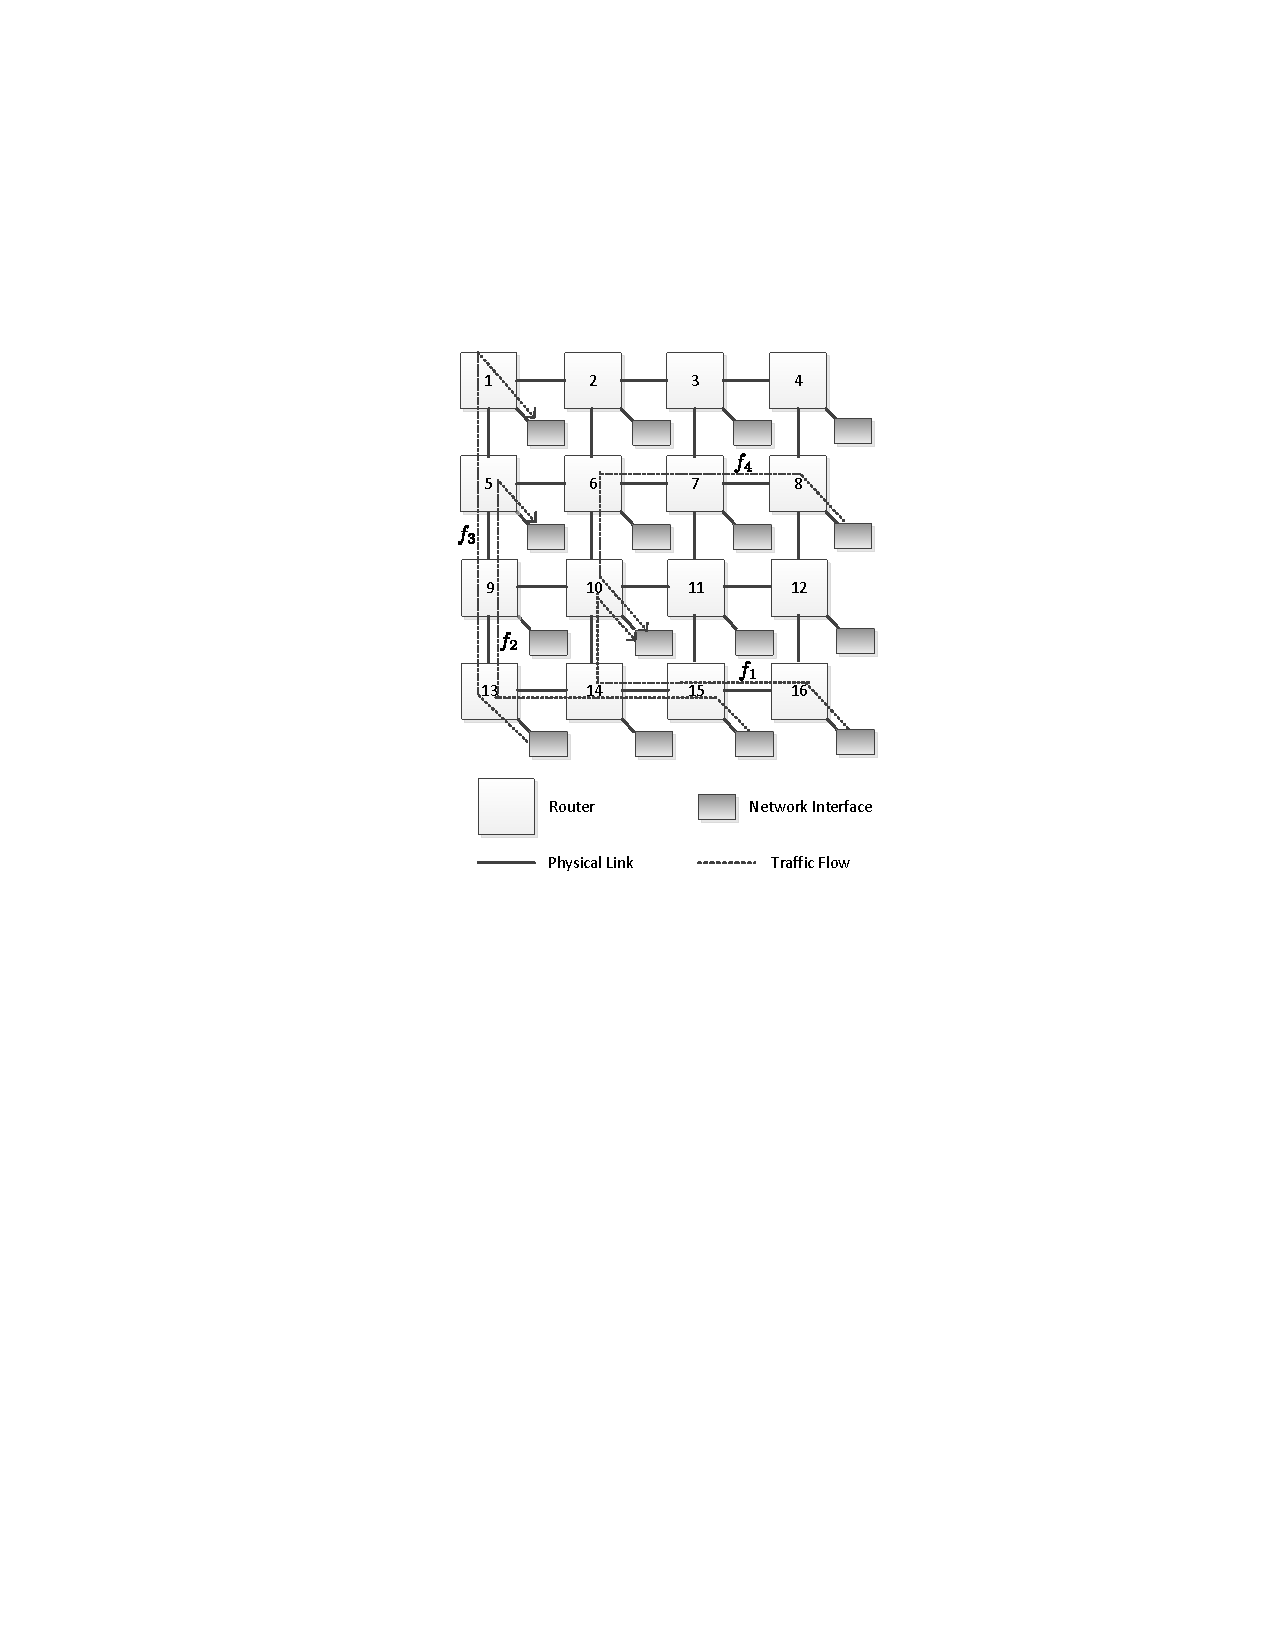
\includegraphics[scale=0.9]{figures/mesh.pdf}\\
  \caption{Mesh topology with 4 real-time traffic flows}\label{topology}
\end{figure}

The entire priority-aware NoC is represented as a directional network topology graph $G:\ V\times E$, where $V$ and $E$ represent the set of routers and links respectively. Each link $e_{i,j}\in E$ corresponds to a physical channel connecting the two routers $R_i$ and $R_j$. A flow is a sequence of packets with the same transmission path, source address and destination address. The path of a flow $f_i$ traversed is defined as a router chain starting from the ingress router (denoted as $start_i$) and ending at the egress router (denoted as $end_i$). The set of all the flows in the network is denoted as $\mathcal{F}$, and each flow $f_i\in\mathcal{F}$ has a fixed-priority $P_i$ and deadline $D_i$. The set of routers along the path of $f_i$ is denoted as $\mathcal{R}_i$, and the set of links a flow $f_i$ traversed is denoted as $\Gamma_i$. There exists interference between flow $f_i$ and $f_j$, if and only if $\Gamma_i\wedge\Gamma_j\neq\emptyset$. For all the router $R_j$ along the path of flow $f_i$, denote the set of contending flows at $R_j$ sharing the same priority with $f_i$ as $\Theta_{R_j,f_i}$, the set of contending flows at $R_j$ with lower priorities as $\Omega_{R_j,f_i}$, and the buffer size as $B_{R_j^{p},f_i}$. In addition, let $M_{R_j,f_i}$ and $N_{R_j,f_i}$ denote the number of flows in $\Omega_{R_j,f_i}$ and $\Theta_{R_j,f_i}$, respectively.

Our algorithms are topology-independent, but to demonstrate the basic idea, we take the mesh topology shown in Fig. \ref{topology} as an example throughout this paper. Routers in the mesh topology have at most five input/output ports, corresponding to the four cardinal directions (West, East, North and South) and the Network Interface (NI), which connects the local Intellectual Property (IP) core. There are four traffic flows in Fig. \ref{topology}, i.e. $f_1$, $f_2$, $f_3$ and $f_4$. We must emphasize that, although there are only four flows in the network, it is sufficient to demonstrate the idea of our method, and our method can handle more traffic flows efficiently. Our method extends the existing methods in \cite{73}\cite{Qian489900} to allow multiple flows share the same priority. Flits of different flows sharing the same priority are served in round-robin order when they are designated the same output port. Since the minimum transmission unit in NoC is flit and a high-priority packet can preempt the transmission of a low-priority packet, the NoC architecture considered in this paper is flit-level preemptive \cite{Lee:2003:RWC:846077.846083}.

\subsection{Introduction to Real-Time Calculus}\label{intrortc}
Real-time calculus \cite{1253607} is the theoretic extension of the DNC theory \cite{Boudec2001Network}, by adding the upper service curve and lower arrival curve to describe the maximum service capacity of a system and the minimum arrival rate of a event stream. It is the mathematical basis of the Modular Performance Analysis (MPA) \cite{Wandeler2006System} technique used for real-time task scheduling. Due to the space limitation, we only present the definitions of the RTC arrival curve and service curve in this subsection. For more details about this theory, please refer to \cite{1253607}.
\begin{definition}[Real-Time Arrival Curve \cite{1253607}]
Let $R[s,t)$ denote the number of events that arrived within the time interval $[s,t)$. The lower and upper bounds on $R[s,t)$ are called the lower arrival curve $\alpha^l$ and upper arrival curve $\alpha^u$ which satisfy
$$\alpha^l(t-s)\leq R[s,t)\leq \alpha^u(t-s),\forall s<t$$
where $\alpha^l(0)=\alpha^u(0)=0$. The RTC arrival curve for a event stream is denoted as $<\alpha^l,\alpha^u>$ for short.
\end{definition}

\begin{definition}[Real-Time Service Curve \cite{1253607}]
Let $S[s,t)$ denote the total number of events that can be processed by the system in the time interval $[s,t)$. The lower and upper bounds on $S[s,t)$ are called the lower service curve $\beta^l$ and upper service curve $\beta^u$ which satisfy
$$\beta^l(t-s)\leq S[s,t)\leq \beta^u(t-s),\forall s<t$$
where $\beta^l(0)=\beta^u(0)=0$. The RTC service curve for a system is denoted as $<\beta^l,\beta^u>$ for short.
\end{definition}

From these two definitions, we find that the upper arrival curve and lower service curve correspond to the arrival curve and service curve of DNC theory \cite{Boudec2001Network}. Similarly, the upper service curve is identical to the maximum service curve of DNC theory. Thus, the two concatenation theorems for service curve (see Theorem 1.46 in \cite{Boudec2001Network}) and maximum service curve (see Theorem 1.6.1 in \cite{Boudec2001Network}) together form the concatenation theorem for the RTC service curve. Assume a event stream traverses two systems $S_1$ and $S_2$ in sequence, and $S_i$ offers an RTC service curve $<\beta^l_i,\beta^u_i>$ $(i=1,2)$ to this event stream. The concatenation theorem gives the equivalent RTC service curve offered by these two systems to this event stream, which is $<\beta^l_1\otimes\beta^l_2,\beta^u_1\otimes\beta^u_2>$.

In this paper, we will utilize the discrete time RTC arrival curve and service curve to characterize the arrived traffic and service capacity, since the minimum time unit in the wormhole-switched NoC is the clock period $T$. Events in arrival curve and service curve refer to the arrival and service of flits, respectively. If we obtain the arrival curve $<\alpha^l,\alpha^u>$ of a specific flow and the service curve $<\beta^l,\beta^u>$ provided to this flow, we can get the output arrival curve $<\alpha^{l^\prime},\alpha^{u^\prime}>$ of this flow and leftover service curve $<\beta^{l^\prime},\beta^{u^\prime}>$ for the other flows with the following equations \cite{1253607}:
\begin{equation}\label{alphal}
\alpha^{l^\prime}=\min\{(\alpha^l\oslash\beta^u)\otimes\beta^l,\beta^l\}
\end{equation}
\begin{equation}\label{alphau}
\alpha^{u^\prime}=\min\{(\alpha^u\otimes\beta^u)\oslash\beta^l,\beta^u\}
\end{equation}
\begin{equation}\label{betal}
\beta^{l^\prime}=(\beta^l-\alpha^u)\bar{\otimes}0
\end{equation}
\begin{equation}\label{betau}
\beta^{u^\prime}=\max\{(\beta^u-\alpha^l)\bar{\oslash}0,0\}
\end{equation}
where $\otimes$, $\oslash$, $\bar{\otimes}$, $\bar{\oslash}$ correspond to the min-plus convolution, de-convolution, and max-plus convolution and de-convolution \cite{Boudec2001Network}.

After we obtain the arrival curve $<\alpha^l_{f},\alpha^u_{f}>$ of flow $f$ and the service curve $<\beta_{R_j,f}^l,\beta_{R_j,f}^u>$ offered by each router $R_j$ ($j=1,2,\cdots,N$) to flow $f$ along its entire path, we can obtain the end-to-end delay bound by the following equation \cite{Boudec2001Network}
\begin{equation}\label{delay}
Delay(f)=H(\alpha^u_{f},\beta^l_{R_1,f}\otimes\beta^l_{R_2,f}\otimes\cdots\otimes\beta^l_{R_N,f})
\end{equation}
where operator $H(\cdot,\cdot)$ means the maximal horizontal deviation between the two operands.

\section{Delay Analysis and Buffer Sizing}\label{modeling}
In this section, we first build an RTC based performance model for the priority-aware wormhole-switched NoC. This model comprises two parts, i.e. traffic model and service model. The traffic model utilizes the RTC arrival curve to describe the arrival process of each flow, and we will introduce two methods to obtain the arrival curve in subsection \ref{traffic}. The service model characterize the services offered by the priority-aware NoC to each flow, which is much more complicated than the traffic model. While constructing the service model, the follow four issues should be considered: (1) Only the head flit needs to traverse the RC and VA stages, because the non-head flits of a packet follow the data-path built by the head flit. To simplify our RTC model, we need a special mechanism to characterize the service offered to head and non-head flits in a unified way. (2) Our model extends the existing approach \cite{73}\cite{Qian489900} by allowing priority sharing among flows. Thus, the leftover service curve provided to the lower-priority flows can only be derived when all the service curves of high-priority flows have been computed. (3) Due to the limited on-chip buffer space, credit-based flow control is used as a back-pressure mechanism to prevent buffer overflow. Before analyzing the end-to-end delay bound with Eq.(\ref{delay}), we should first break the cyclic-dependence between the adjacent routers caused by flow control. (4) To guarantee the tightness of performance bounds and simplify the numerical computation, we should apply the concatenation theorems as much as possible before deriving the leftover service curve. But, this process becomes complicated when the credit-based flow control is taken into consideration. We will discuss the first two issues in subsection \ref{router}, and the last two issues are discussed in subsection \ref{flowcontrol} and subsection \ref{csp}, respectively. Based on the proposed performance model, we propose an end-to-end delay analysis algorithm and a buffer sizing algorithm, as presented in subsection \ref{e2elatency} and subsection \ref{bufferopt}, respectively.

\subsection{Traffic Model}\label{traffic}
The communication in a priority-aware wormhole-switched NoC is realized by transmitting packets, and the packet is further divided into flits, which is the minimum transmission unit in wormhole-switched NoC. Denote by $<\alpha^l(\Delta),\alpha^u(\Delta)>$ the flit arrival curve of a flow, namely, the minimum and maximum number of flits can be seen within any time window of width $\Delta$. We can extract the flit arrival curve from the synthetic traffic or communication trace with the sliding window method \cite{1253607}. For each window size $\Delta$, this method tries to find the maximal and minimal number of arrived flits (corresponding to $\alpha^l(\Delta)$ and $\alpha^u(\Delta)$) by analyzing the time series of flits. The synthetic traffic or communication trace is not required to be periodic, since the RTC theory makes no assumption on the periodicity of the traffic. However, the obtained flit arrival curve can only be applied to compute the worst-case performance bound at the flit level. To obtain the packet level delay bound, this arrival curve must be $L$-packetized \cite{Boudec2001Network}. Denote by $L(n)$ the cumulative packet length\footnote{Let $l_i$ be the length (in flits) of $i$-th packet, the cumulative packet length $L(n)$ is defined as $L(n)=\sum_{i=1}^n l_i$.} of the first $n$ packets in a flow, $R(t)$ the cumulative arrived flits by time $t$. Then, the $L$-packetizer operator $\mathcal{P}^l(\cdot)$ is defined as $\mathcal{P}^L(R(t))=\underset{n\in\mathcal{N}}{\sup}\{L(n)1_{L(n)\leq R(t)}\}$\footnote{$\mathcal{N}$ is the set of natural numbers and $1_{\{val\}}$ is the indicator function, $1_{\{val\}}=1$ if and only if $val$ is true.}. Intuitively, $\mathcal{P}^l(\cdot)$ can be interpreted as the largest cumulative packet length contained in $R(t)$, as shown in Fig. \ref{lpkt}. Denote by $L_{max}$ the maximum packet length (in flits) of a flow, according to the basic properties of $L$-packetizer \cite{Boudec2001Network}, we have
$$R(t)-l_{max}\leq \mathcal{P}^L(R(t))<R(t)$$
and
$$R(s)-l_{max}\leq \mathcal{P}^L(R(s))<R(s)$$
which indicate
$$\alpha(t-s)^l-l_{max}<\mathcal{P}^L(R(t))-\mathcal{P}^L(R(s))<\alpha(t-s)^u+l_{max}.$$
The inequalities above mean that, if a flow has a flit arrival curve $<\alpha^l(\Delta),\alpha^u(\Delta)>$, the $L$-packetized flow has a packet arrival curve $<\alpha^l(\Delta)-l_{max}1_{\{\Delta>0\}},\alpha^u(\Delta)+l_{max}1_{\{\Delta>0\}}>$. We can also directly obtain the $L$-packetized arrival curve instead of transformation from flit arrival curve for some special cases. For example, suppose all the packets in a flow have the same length $F$ and arrived periodically with period $I$. We can obtain the flit arrival curve of this flow by applying the sliding window method, as shown in Fig. \ref{perio}. The obtained flit arrival curve is equivalent to the $L$-packetized arrival curve $\mathcal{P}^L(\alpha)$, since $\mathcal{P}^L(R(t))=R(t)$ and $\mathcal{P}^L(\alpha(t))=\alpha(t)$.
\begin{figure}
  \centering
  \subfloat[]{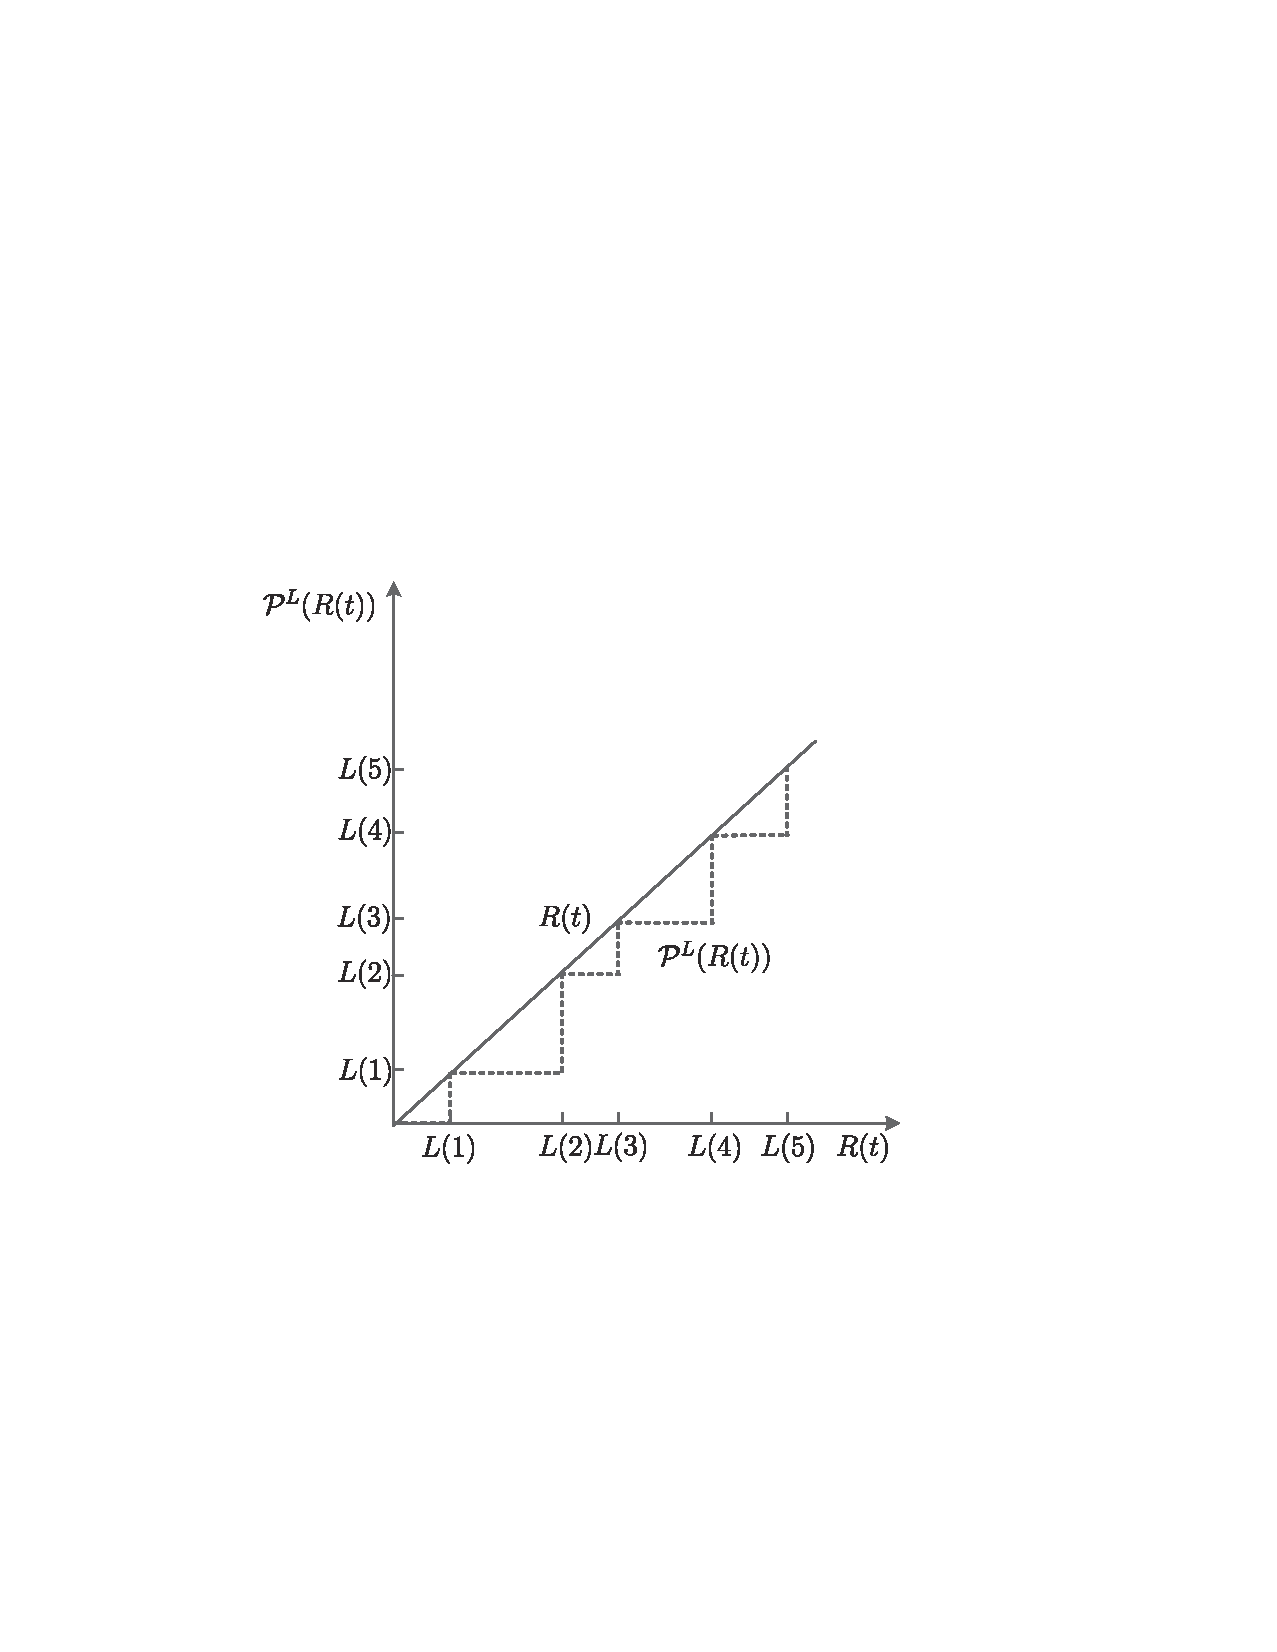
\includegraphics[scale=0.35]{figures/LPKT.pdf}\label{lpkt}}\hspace{10pt}
  \subfloat[]{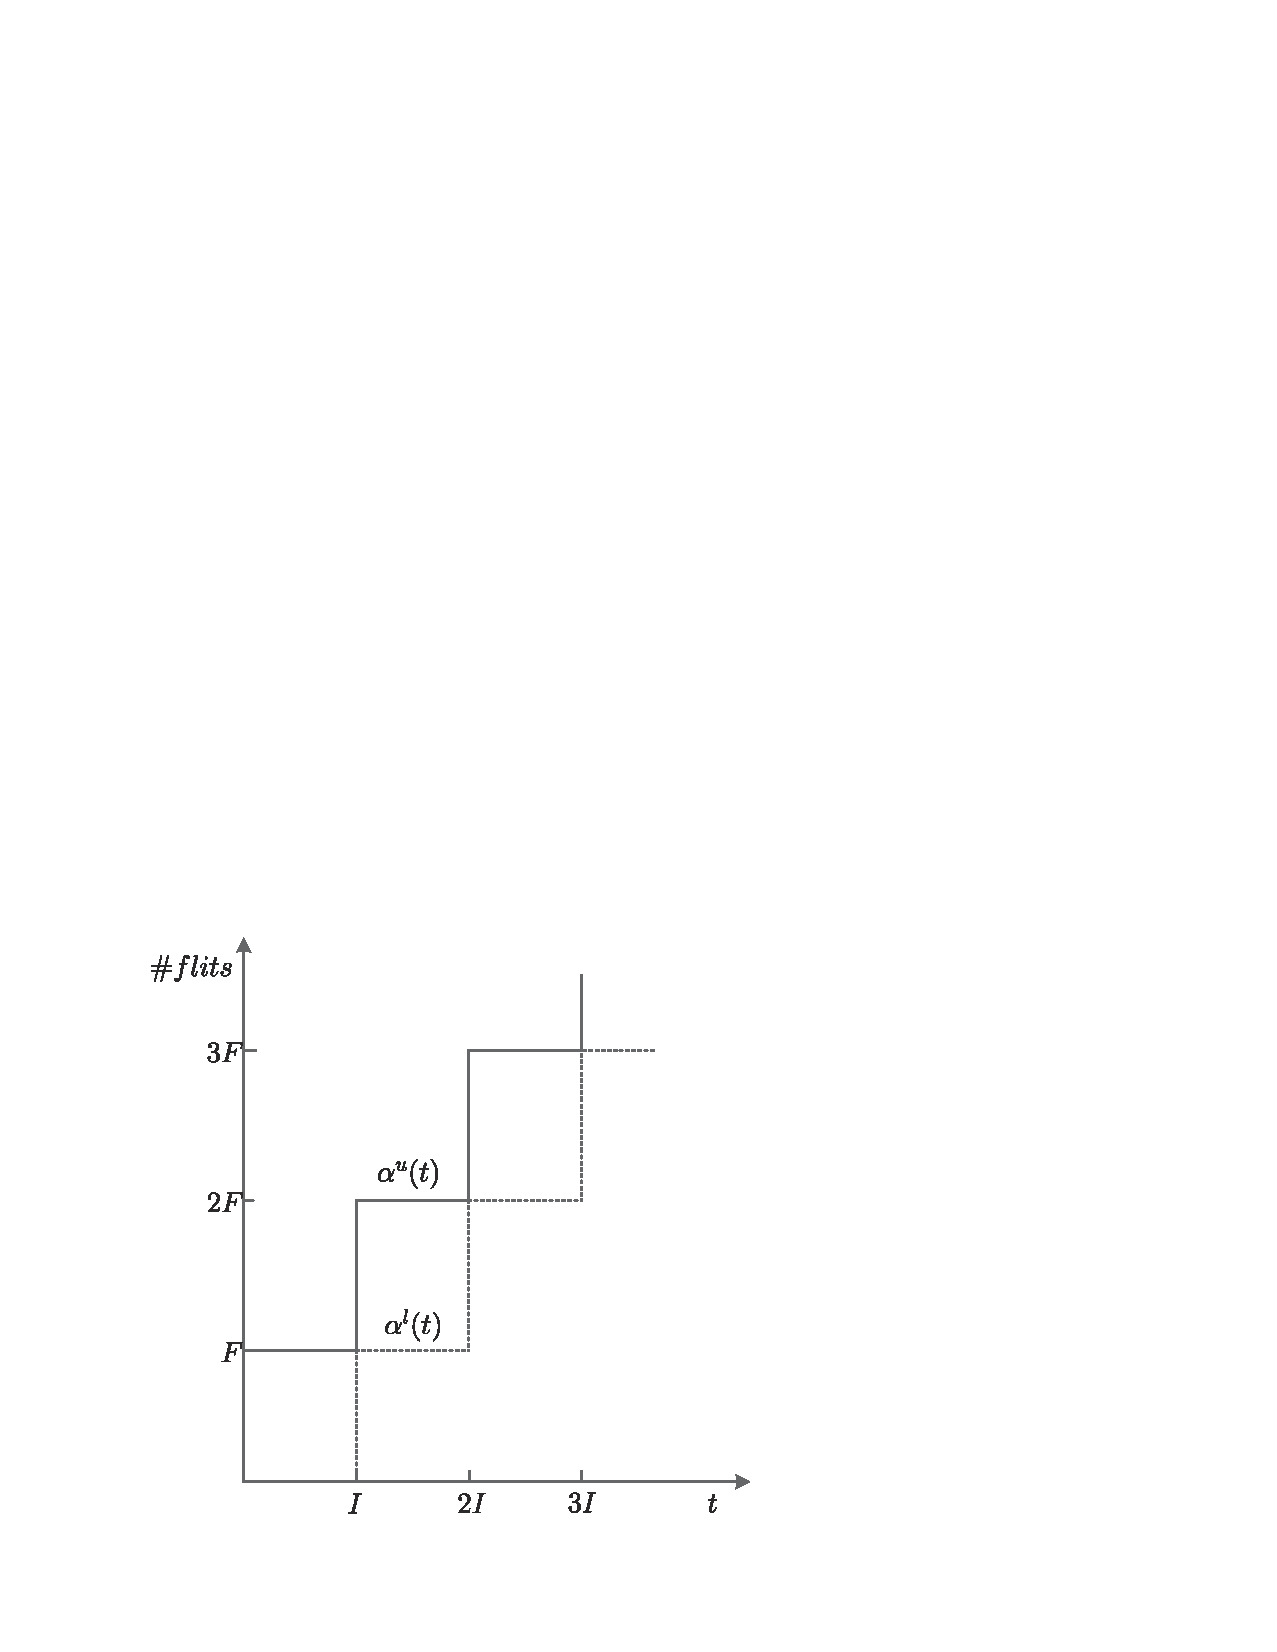
\includegraphics[scale=0.35]{figures/AC.pdf}\label{perio}}
  \caption{Traffic model. (a) Definition of $\mathcal{P}^L(R(t))$. Cumulative arrival function $R(t)$ and the $L$-packetized cumulative arrival function $\mathcal{P}^L(R(t))$ are represented by the dotted line and solid line, respectively. (b) Real-time calculus arrival curve for periodically arrived traffic with period $I$ and packet length $F$. The solid line and dotted line represent the upper arrival curve and lower arrival curve.}\label{ac}
\end{figure}

\subsection{Service Model}\label{router}
While modeling the service capacity of routers with RTC, we can analyze the data-path of a flow stage-by-stage. On obtaining the service curve for each stage, the service curve provided by the router to the flow can be obtained by concatenating all the service curves of these five stages. This is significantly different from the existing DNC based model \cite{qian2009analysis,Qian489900}, where they treat the entire router as a whole and designate a Latency-Rate (LR) service curve \cite{Boudec2001Network} for simplicity. The advantage of our method is that, it can be easily modified to characterize the non-standard router micro-architectures, by simply letting the service curve of non-existed stages to be a burst delay function $\delta_0(t)$\footnote{$\delta_{val}(t)=+\infty$ if $t>val$, and 0 otherwise.}. Next, we try to obtain the service curves of all these five stages:
\begin{figure}
  \centering
  \subfloat[]{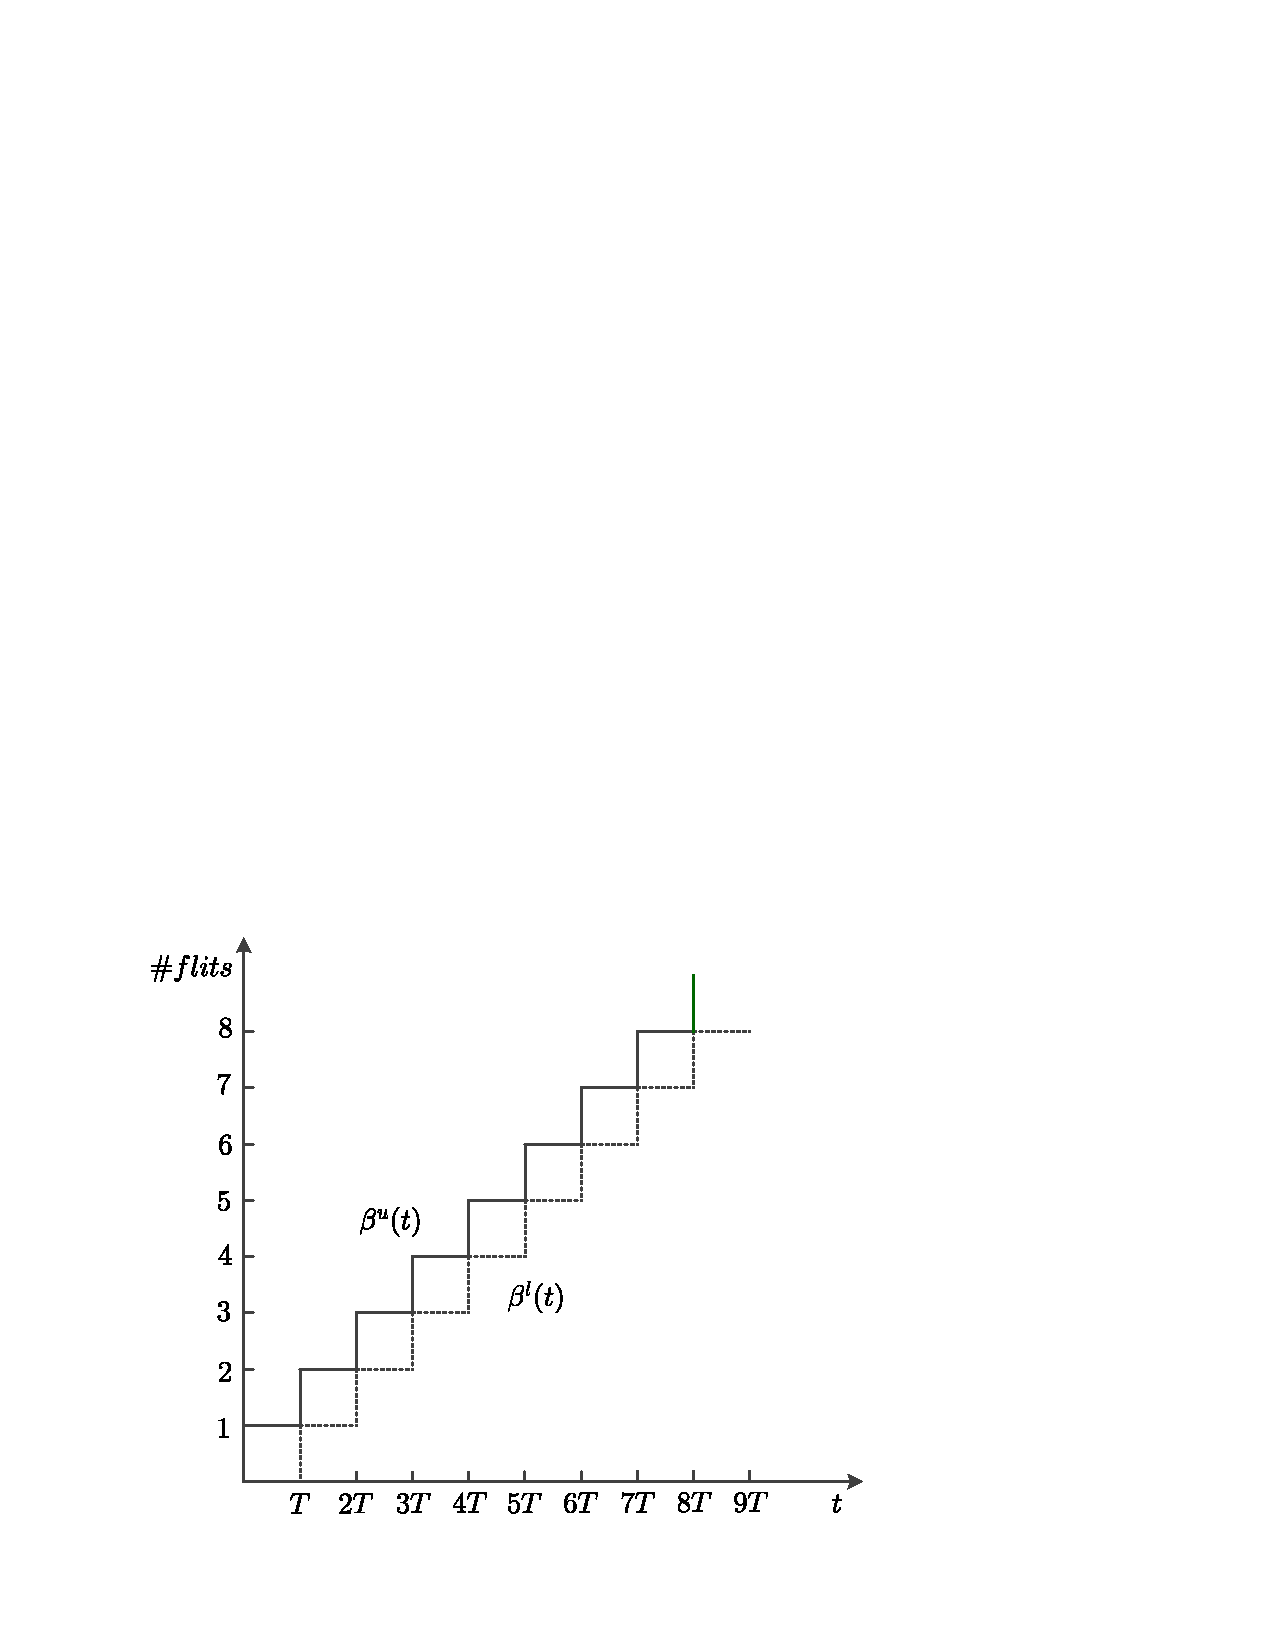
\includegraphics[scale=0.35]{figures/BW_ST_SA.pdf}\label{result1}}\hspace{10pt}
  \subfloat[]{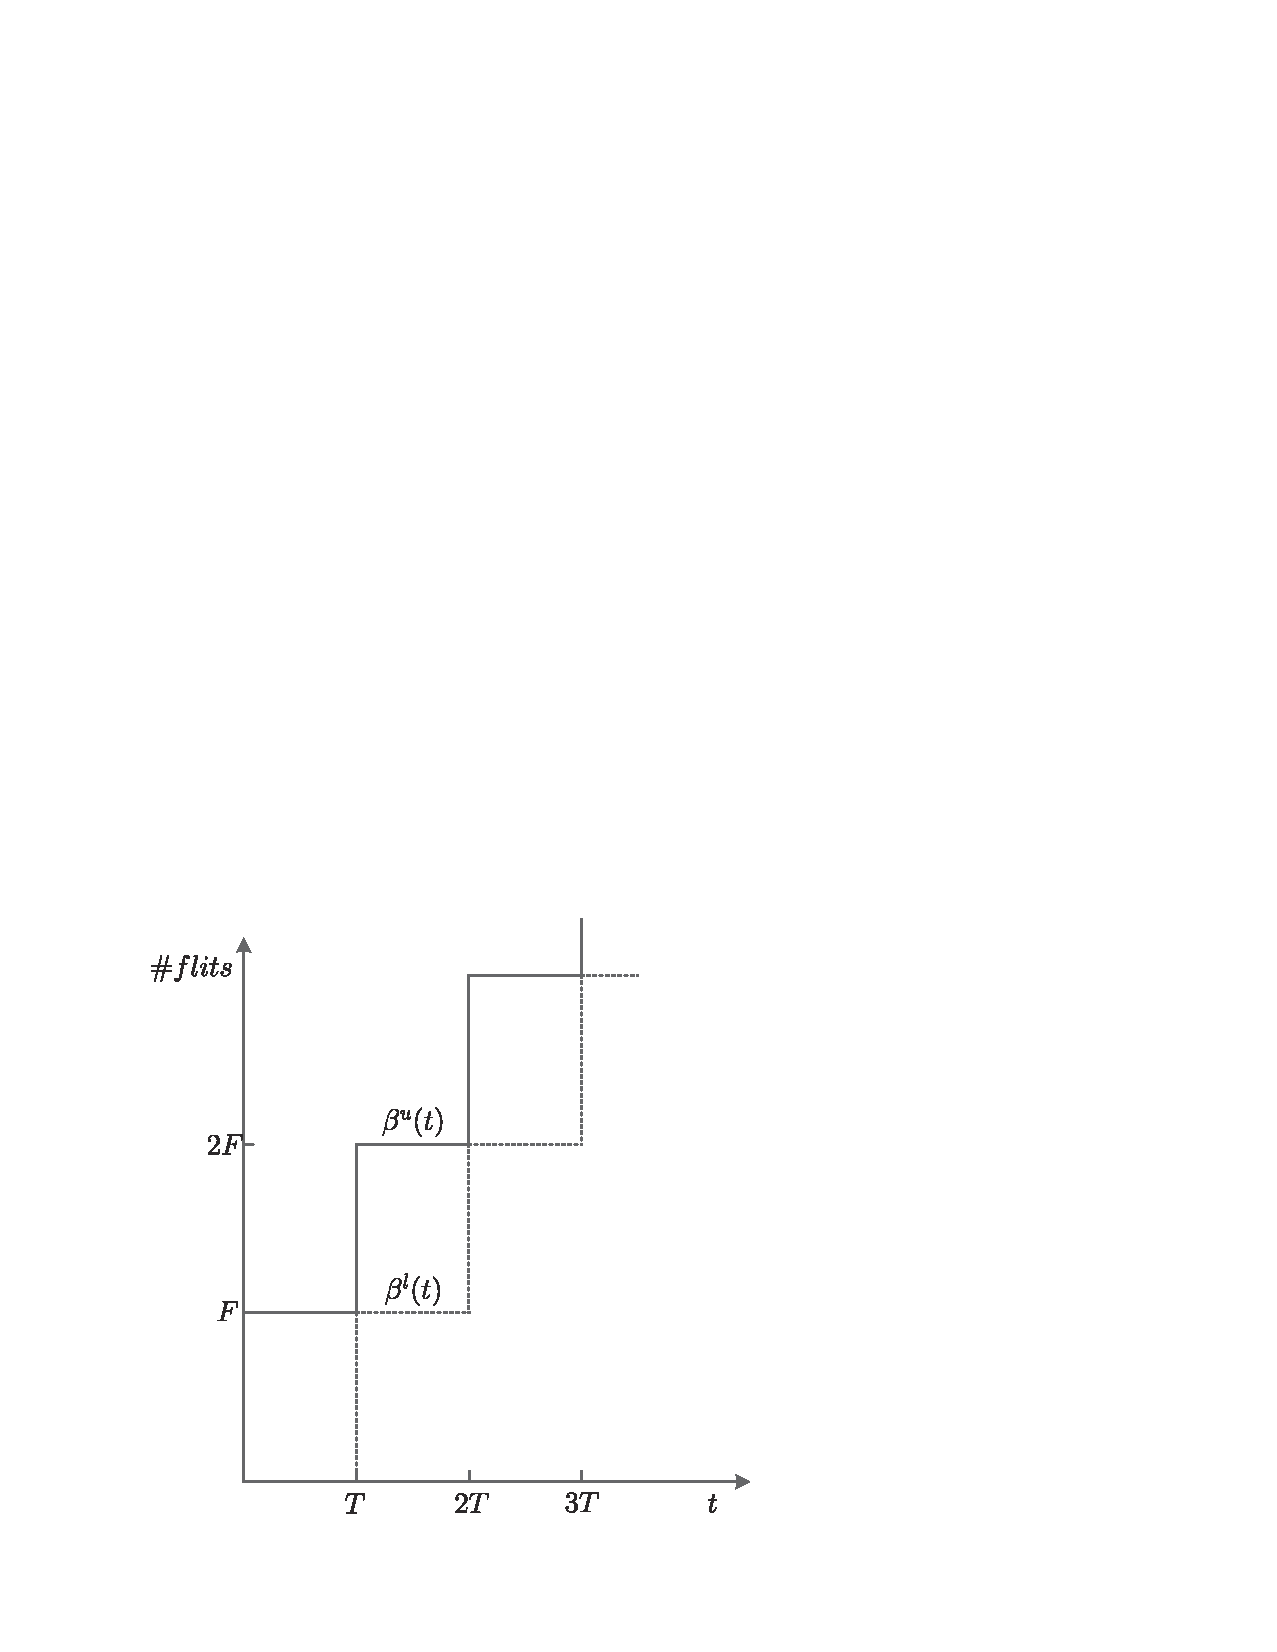
\includegraphics[scale=0.35]{figures/RC_VA.pdf}\label{result2}}
  \caption{Service model for each pipeline stage. The solid lines and dotted lines represent the upper service curves and lower service curves, respectively. (a) Service curve of BW, SA and ST stages; (b) Service curve of RC and VA stages.}
\end{figure}

(1) BW stage and ST stage: all the flits within a traffic flow will traverse these two stages, and experience a fixed delay $T$. Take the BW stage as an example, for any time interval of length less than $T$, the maximum and minimum number of flits can be served are one and zero, respectively, since it outputs one flit at each cycle $T$. Similarly, for any time interval of length greater than $T$, the maximum and minimum number of flits that can be seen are two and one, respectively. The resulted service curves, i.e. $<\beta^l_{BW},\beta^u_{BW}>$ and $<\beta^l_{ST},\beta^u_{ST}>$, are shown in Fig. \ref{result1}.

(2) RC stage and VA stage: the traverse latency of head flit and non-head flits at these two stages are $T$ and 0, respectively. A sophisticated solution to construct a unified service curve for head flit and non-head flits at these two stages comes from recognizing that these two stages can service an entire packet within $T$ period. Suppose the packet length is $F$, the equivalent service curve for these two stages, i.e. $<\beta^l_{RC},\beta^u_{RC}>$ and $<\beta^l_{VA},\beta^u_{VA}>$, can be easily obtained by amplifying the service curve of Fig. \ref{result1} in $y$-axis by a factor $F$, as shown in Fig. \ref{result2}.

(3) SA stage: each output port of the wormhole-switched NoC has a switch allocator to schedule the switch traversal among all the contending flows at each clock cycle. Thus, following the same procedure as BW and ST stage, we can get the service curves provided by the switch allocators at each output port to all the contending flows, as shown in Fig. \ref{result1}. We also define the notation $<\beta_{SA,R_i^{p}}^l,\beta_{SA,R_i^{p}}^u>$ to distinguish the service curve of switch allocator at specific output port from the others. For the mesh topology, the port indicator $p$ can be concreted with $W$ (West port), $E$ (East port), $S$ (South port) and $N$ (North port) or $L$ (Local port).

Alert readers have noticed that, the contention of different flows only occurs at SA stage. For the fixed-priority based scheduling policy, switch allocators provide services for high-priority flows first, and flows with the same priority will be served with Round-Robin order. The unserved flows will be imposed an additional latency $T$ due to the failure of switch arbitration. Thus, if we obtained the service curve provided by SA stage to flow $f_j$, we can obtain the service curve of the router directly.

Denote by $<\beta_{SA,R_i^{p},f_j}^l,\beta_{SA,R_i^{p},f_j}^u>$ the service curve provided to flow $f_j$ by SA stage of router $R_i$, the equivalent service curve of router $R_i$ provided to $f_j$, i.e. $<\beta_{R_i^{p},f_j}^l,\beta_{R_i^{p},f_j}^u>$, can be obtained by concatenating the service curves of all the five stages together:
$$\beta_{R_i^{p},f_j}^l=\beta_{BW}^l\otimes\beta_{RC}^l\otimes\beta_{VA}^l\otimes\beta_{SA,R_i^{p},f_j}^l\otimes \beta_{ST}^l,$$
$$\beta_{R_i^{p},f_j}^u=\beta_{BW}^u\otimes\beta_{RC}^u\otimes\beta_{VA}^u\otimes\beta_{SA,R_i^{p},f_j}^u\otimes \beta_{ST}^u.$$

Suppose the total service curve provided by a switch allocator is $<\beta_{SA,R_i^{p}}^l,\beta_{SA,R_i^{p}}^u>$ and the leftover service curve after serving the flows with higher priority than $f_j$ is $<\beta_{SA,R_i^{p}}^{l^\prime},\beta_{SA,R_i^{p}}^{u^\prime}>$, in order to obtain the service curve $<\beta_{SA,R_i^{p},f_j}^l,\beta_{SA,R_i^{p},f_j}^u>$, we should consider the following two cases:

(a) All the flows contending with $f_j$ at $R_i$ have lower priorities. For the synchronized router architecture, flow $f_j$ gets the total leftover service curve $<\beta_{SA,R_i^{p}}^{l^\prime},\beta_{SA,R_i^{p}}^{u^\prime}>$.

(b) There exists some contention flows with the same priority as $f_j$. Denote by $\Theta_{R_i,f_j}$ the set of contention flows at router $R_i$ with the same priority as $f_j$, and let $N_{R_i,f_j}$ be the number of flows in $\Theta_{R_i,f_j}$. Since all the flows in $\Theta_{R_i,f_j}$ got serviced in Round-Robin order, the service curve provided to $f_j$ is $<\lfloor\beta^{l^\prime}_{SA,R_i^{p}}/(N_{R_i,f_j}+1)\rfloor,\lceil\beta^{u^\prime}_{SA,R_i^{p}}/(N_{R_i,f_j}+1)\rceil>$, where $\lceil\cdot\rceil$ and $\lfloor\cdot\rfloor$ are the ceiling operator and flooring operator, respectively. After serving all the flows in $\Theta_{R_i,f_j}$, the leftover service curve for low-priority flows can be obtained by applying Eq.(\ref{betal}) and Eq.(\ref{betau}).

\subsection{Upper Service Curve of Flow Controller}\label{flowcontrol}
Credit-based flow control introduces cyclic-dependence between the adjacent routers, and leads to self-blocking within a flow due to the insufficiency of buffer space at the downstream router. To make the discussion concrete, we take flow $f_2$ as an example and utilize the scheduling network model \cite{1253607} in RTC theory to visualize the credit-based flow control and complex relationship among $f_2$ and the other flows, as shown in Fig. \ref{f2}. We ignore flow $f_4$ and the flow control of the other flows for clarity. We also assume that, all the destination IP cores can consume the ejected flits immediately, thus there is no flow control between the ejection router and destination NI. However, to prevent the buffer overflow, the flow control between source NI and injection router is necessary. The flow control mechanism introduces a feedback control loop between adjacent routers, preventing us from deriving the performance bound directly even after we have obtained the service curve reserved at each router for the target flow. Historically, this issue is addressed  by fixed-point iteration \cite{schioler2005network} or transformation from marked dataflow graph \cite{Thiele:2009:MPA:1629335.1629353}. In this paper, we try to tackle the same problem with another solution. This is motivated by \cite{qian2009analysis}, where the authors abstract the flow control as a network element (called flow controller) providing a service curve $\beta_{\tau}$ (corresponding to the lower service curve of RTC theory). Then, this service curve is obtained by applying some basic properties of DNC theory \cite{Boudec2001Network}.
\begin{figure*}
  \centering
  % Requires \usepackage{graphicx}
  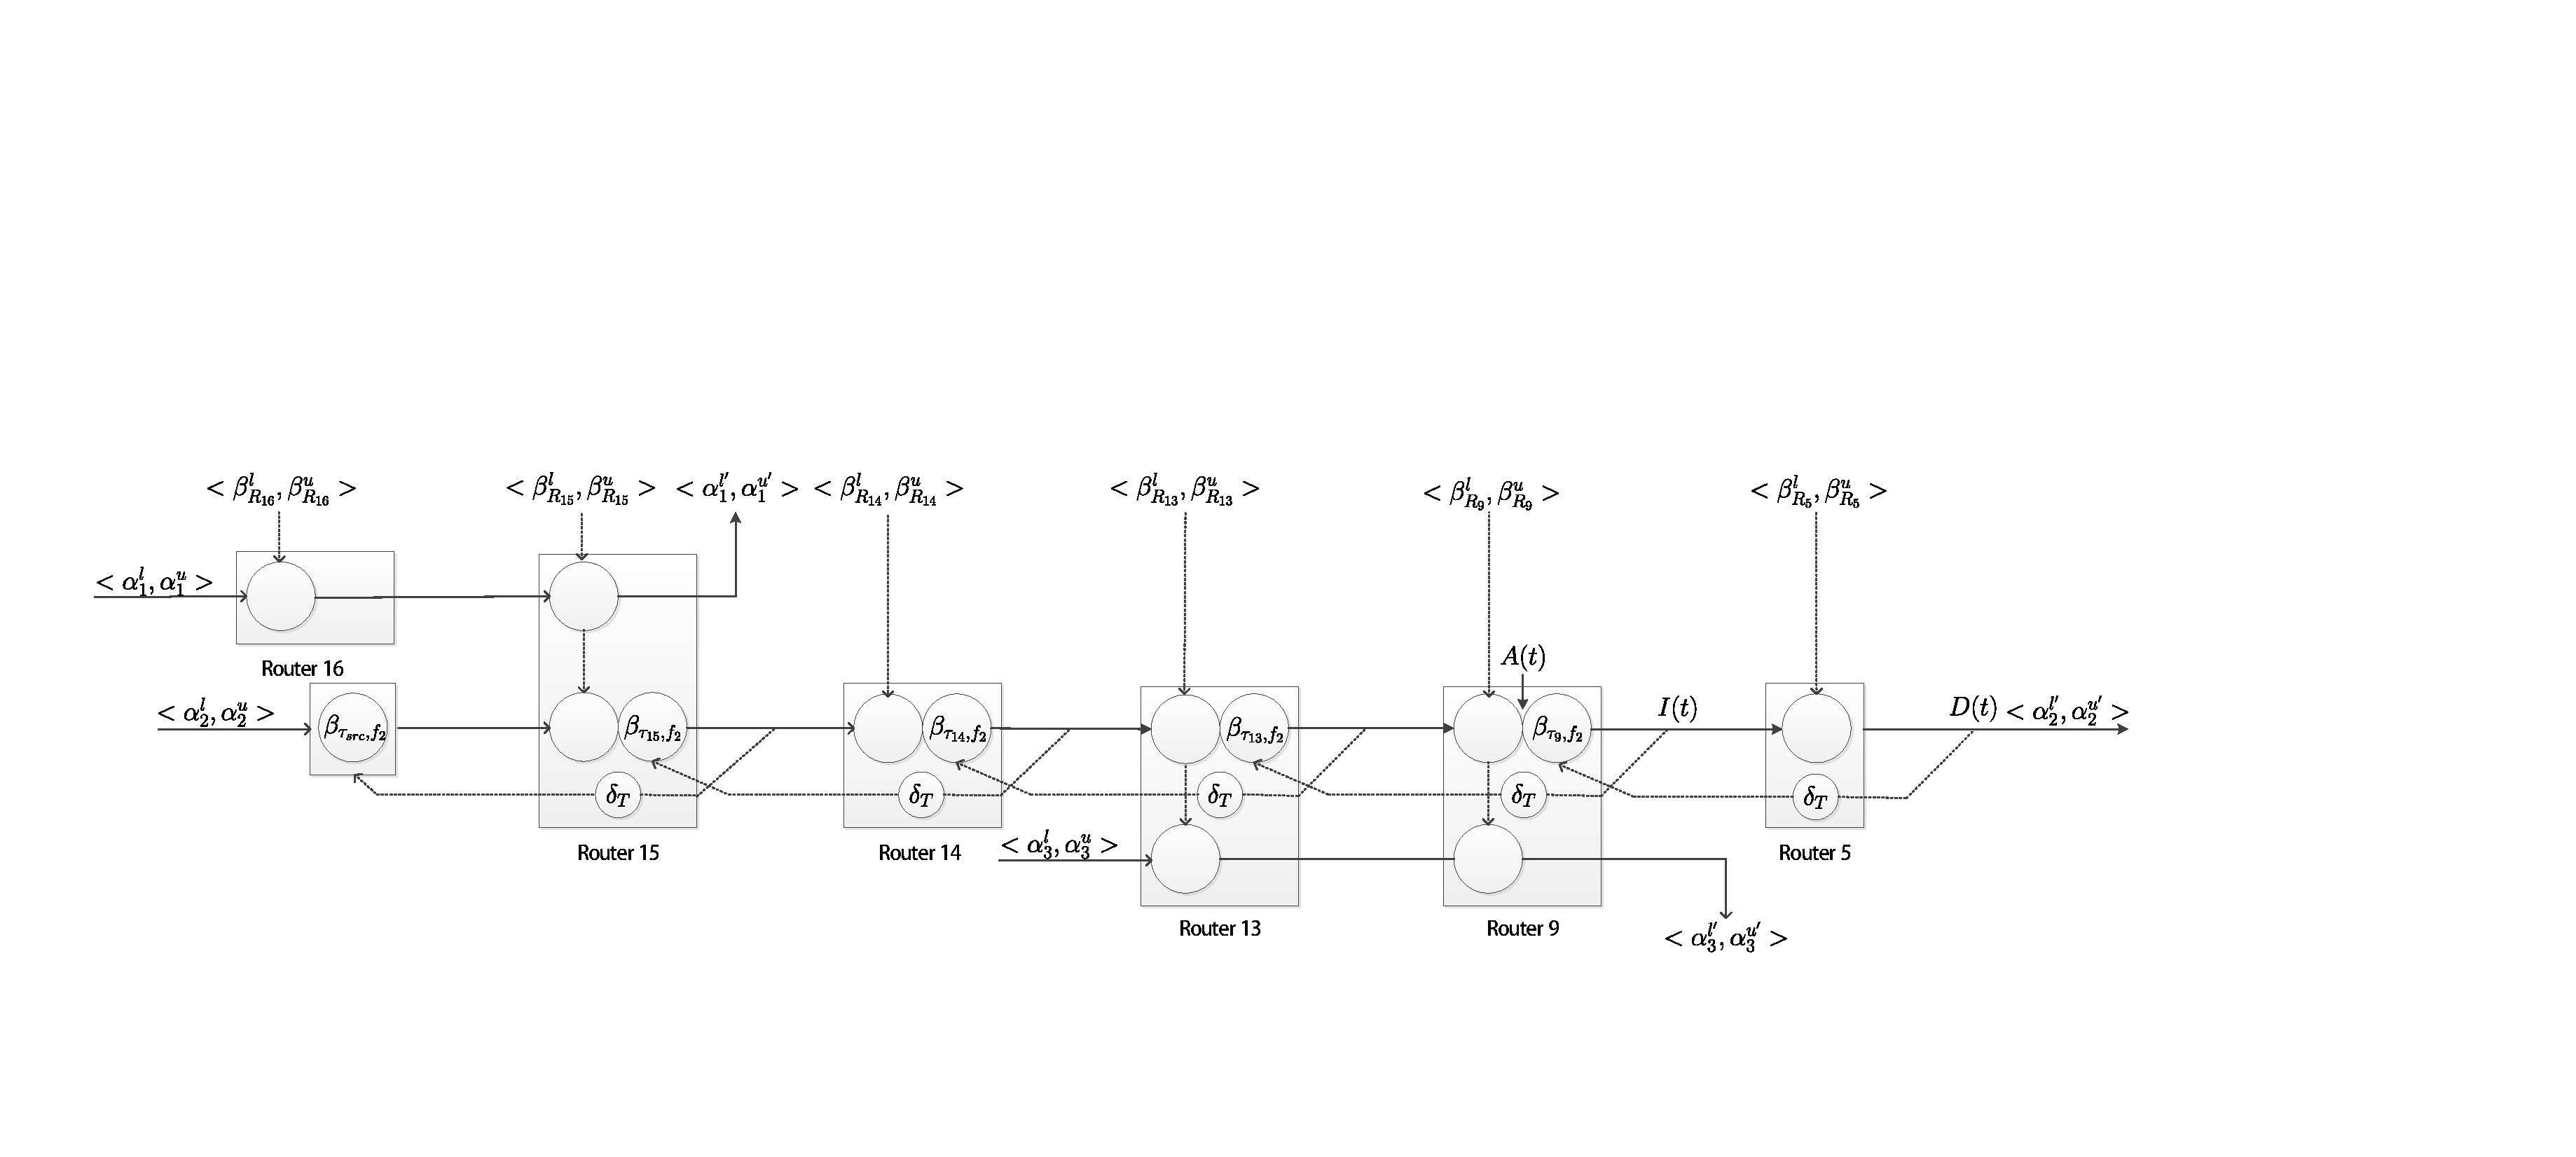
\includegraphics[scale=0.35]{figures/f2.pdf}\\
  \caption{Scheduling network model for flow $f_2$}\label{f2}
\end{figure*}

In this subsection, we follow the similar procedure as \cite{qian2009analysis} to derive the upper service curve for the flow controller, as summarized in Theorem \ref{credit}. The obtained upper service curve together with the lower service curve derived in \cite{qian2009analysis} enable us to break the cyclic-dependences caused by flow control and build a comprehensive performance model with RTC.
\begin{theorem}\label{credit}
Suppose the router provides an RTC service curve $<\beta^l,\beta^u>$, the buffer size and credit feedback delay are denoted as $B$ and $\sigma$, respectively. Then, the flow controller provides an equivalent RTC service curve $<\overline{\beta^l\otimes\delta_\sigma(t)+B},\overline{\beta^u\otimes\delta_\sigma(t)+B}>$, where $\bar{f}$ is the sub-additive closure of $f$ \cite{Boudec2001Network}.
\end{theorem}
\begin{IEEEproof}
The lower service curve has been derived in \cite{qian2009analysis}. In the rest of this proof, we will take the flow control between $R_9$ and $R_5$ in Fig. \ref{f2} as an example to derive the upper service curve. Denote the amount of injected and departed flits at $R_5$ by time $t$ as $I(t)$ and $D(t)$, and the amount of flits served by $R_9$ by time $t$ as $A(t)$. The feedback link can be represented as a network element providing upper service curve $\delta_\sigma(t)$.

For the flow control between router $R_9$ and $R_5$, we have $I(t)\leq A(t)$ for causality and $I(t)\leq D^\prime(t)+B$ due to the effect of flow control, where $D^\prime\leq D\otimes\delta_\sigma$. Thus, $$I(t)\leq\min\{A(t),D^\prime(t)+B\}.$$

Based on the equivalent definition of upper service curve\footnote{please refer to definition 1.6.1 in \cite{Boudec2001Network} for more details.}, we have
$$D(t)\leq I\otimes \beta_{R_5^L,f_2}^u(t).$$

Bring $I(t)$ and $D^\prime(t)$ into this equality, we get
\begin{eqnarray*}
D(t)&\leq& I\otimes \beta_{R_5^L,f_2}^u(t)\\
&\leq& \min\{A\otimes \beta^u_{R_5^L,f_2}(t),D\otimes\delta_\sigma\otimes \beta_{R_5^L,f_2}^u(t)+B\}.
\end{eqnarray*}

By applying Theorem 4.31 in \cite{Boudec2001Network}, we have
$$D\leq A\otimes \beta^u_{R_5^L,f_2}\otimes\overline{\beta_{R_5^L,f_2}^u\otimes\delta_\sigma+B}.$$

Thus,
\begin{eqnarray*}
  I&\leq& \min\{A,D^\prime+B\}\\
  &\leq& \min\{A,D\otimes\delta_\sigma+B\}\\
  &\leq& \min\{A,A\otimes \beta_{R_5^L,f_2}^u\otimes\overline{\beta_{R_5^L,f_2}^u\otimes\delta_\sigma+B}\otimes\delta_\sigma+B\}\\
%  &=& \min\{A\otimes \delta_\sigma,A\otimes (\beta_{R_5^L,f_2}^u\otimes\delta_\sigma+B)\otimes\overline{\delta_\sigma\otimes\beta_{R_5^L,f_2}^u+B}\}\\
  &=& \min\{A\otimes \delta_\sigma,A\otimes \overline{\delta_\sigma\otimes\beta_{R_5^L,f_2}^u+B}\}\\
  &=& A\otimes\min\{\delta_\sigma,\overline{\beta_{R_5^L,f_2}^u\otimes\delta_\sigma+B}\}\\
  &=& A\otimes\overline{\beta_{R_5^L,f_2}^u\otimes\delta_\sigma+B}
\end{eqnarray*}
where the steps from the third line to the fifth line holds due to the general properties of $\otimes$ operator (see Rule 6 and Rule 7 of Theorem 3.1.5 in \cite{Boudec2001Network} for more details), and the last step follows from the definition of sub-additive closure.

The inequality $I\leq A\otimes \overline{\beta_{R_5^L,f_2}^u\otimes\delta_\sigma+B}$ implies that the flow controller between $R_9$ and $R_5$ provides an equivalent upper service curve $\overline{\beta_{R_5^L,f_2}^u\otimes\delta_\sigma+B}$. Thus, we can conclude that for any router providing upper service curve $\beta^u$, the corresponding flow controller has an equivalent upper service curve $\beta^{u}_\tau(t)=\overline{\beta^u\otimes\delta_\sigma(t)+B}$.
\end{IEEEproof}

Theorem \ref{credit} derives the RTC service curve of a single flow controller, and we can get the service curves of all the flow controllers along the router chain of any flow by applying Theorem \ref{credit} iteratively. As shown in Fig. \ref{f2}, the service curve of a flow controller is determined by the service curves of the downstream flow controllers and routers. Hence, for each flow, we should compute the service curves of flow controllers from the ejection router to the injection router. Take flow $f_2$ as an example, we should first compute the service curve of flow controller between $R_5$ and $R_{9}$ (denoted as $<\beta_{\tau_9,f_2}^l,\beta_{\tau_9,f_2}^u>$), which is $<\overline{\beta_{R_5^L,f_2}^l\otimes\delta_\sigma+B},\overline{\beta_{R_5^L,f_2}^u\otimes\delta_\sigma+B}>$. Then, By applying the concatenation theorem, we can obtain the equivalent service curve provided to $f_2$ by router $R_{9}$, i.e. $<\beta_{R_9^N,f_2}^l\otimes\beta_{\tau_9,f_2}^l,\beta_{R_9^N,f_2}^u\otimes\beta_{\tau_9,f_2}^u>$, which can be utilized to derive $<\beta_{\tau_{13},f_2}^l,\beta_{\tau_{13},f_2}^u>$ further. Follow the same procedure, $<\beta_{\tau_{14},f_2}^l,\beta_{\tau_{14},f_2}^u>$, $<\beta_{\tau_{15},f_2}^l,\beta_{\tau_{15},f_2}^u>$ and $<\beta_{\tau_{src},f_2}^l,\beta_{\tau_{src},f_2}^u>$\footnote{$<\beta_{\tau_{src},f_2}^l,\beta_{\tau_{src},f_2}^u>$ denotes the service curve of flow controller between source NI and injection router, as shown in Fig.\ref{f2}.} can be derived iteratively.

\subsection{Collapsible Sub-Path}\label{csp}
To this end, we have built the traffic model, service model and flow control model. Before giving the delay analysis algorithm, we first consider the follow scenario. Flow $f_2$ and $f_3$ in Fig. \ref{topology} contend the output link at both router $R_{13}$ and $R_{9}$. Suppose $P_2>P_3$ and denote by $B_{R_9^N,f_2}$ the buffer size of router $R_{9}$ allocated to flow $f_2$, $<\beta_{R_{13}^N,f_2}^l,\beta_{R_{13}^N,f_2}^u>$ and $<\beta_{R_{9}^N,f_2}^l,\beta_{R_{9}^N,f_2}^u>$ the service curves provided to flow $f_2$ by router $R_{13}$ and $R_{9}$, $<\beta_{\tau_{13},f_2}^l,\beta_{\tau_{13},f_2}^u>$ the service curve for flow controller of router $R_{13}$, $<\alpha_{R_{13},f_2}^l,\alpha_{R_{13},f_2}^u>$ and $<\alpha_{R_{13},f_3}^l,\alpha_{R_{13},f_3}^u>$ the arrival curve of $f_2$ and $f_3$ at router $R_{13}$. The question is: when $B_{R_9^N,f_2}$ is large enough so that $\beta_{R_{13}^N,f_2}^l\otimes\beta_{\tau_{13},f_2}^l=\beta_{R_{13}^N,f_2}^l$ and $\beta_{R_{13}^N,f_2}^u\otimes\beta_{\tau_{13},f_2}^u=\beta_{R_{13}^N,f_2}^u$, how to derive the leftover service curve for $f_3$ at $R_{13}$ and $R_9$, and obtain a tight delay bound of $f_3$ efficiently?

An intuitive solution is: First, obtain the leftover service curve of $R_{13}$ by applying Eq.(\ref{betal}) and Eq.(\ref{betau}). Second, derive the output arrival curve $<\alpha_{R_{9},f_2}^{l^\prime},\alpha_{R_{9},f_2}^{u^\prime}>$ of $f_2$ by applying Eq.(\ref{alphal}) and Eq.(\ref{alphau}). Third, the leftover service curve of $R_9$ can be easily obtained by applying Eq.(\ref{betal}) and Eq.(\ref{betau}). Finally, the equivalent service curve of $f_3$ obtained at $R_{13}$ and $R_9$ can be easily obtained by concatenating these two service curves. Another solution is that we can substitute $R_{13}$ and $R_{9}$ by a virtual router $R_{13,9}$ providing service curve $<\beta_{R_{9}^N,f_2}^l\otimes\beta_{R_{13}^N,f_2}^l,\beta_{R_{9}^{p},f_2}^u\otimes\beta_{R_{13}^N,f_2}^u>$, since $B_{R_9^N,f_2}$ is sufficiently large, and the flow control between $R_{13}$ and $R_9$ can be neglected, as shown in Fig. \ref{collapse}. Then, the service curve of $f_3$ obtained at the virtual router $R_{13,9}$ can be directly obtained by applying Eq.(\ref{betal}) and Eq.(\ref{betau}). Compared with previous router-by-router calculation method, it eliminates the calculation of intermediate arrival curve, and computes the equivalent service curve by invoking Eq.(\ref{betal}) and Eq.(\ref{betau}) just once, which is of computationally efficient. We formalize this observation and propose the concept of Collapsible Sub-Path (CSP) to simplify the calculation and improve the tightness of the delay bound.
\begin{figure}
  \centering
  % Requires \usepackage{graphicx}
  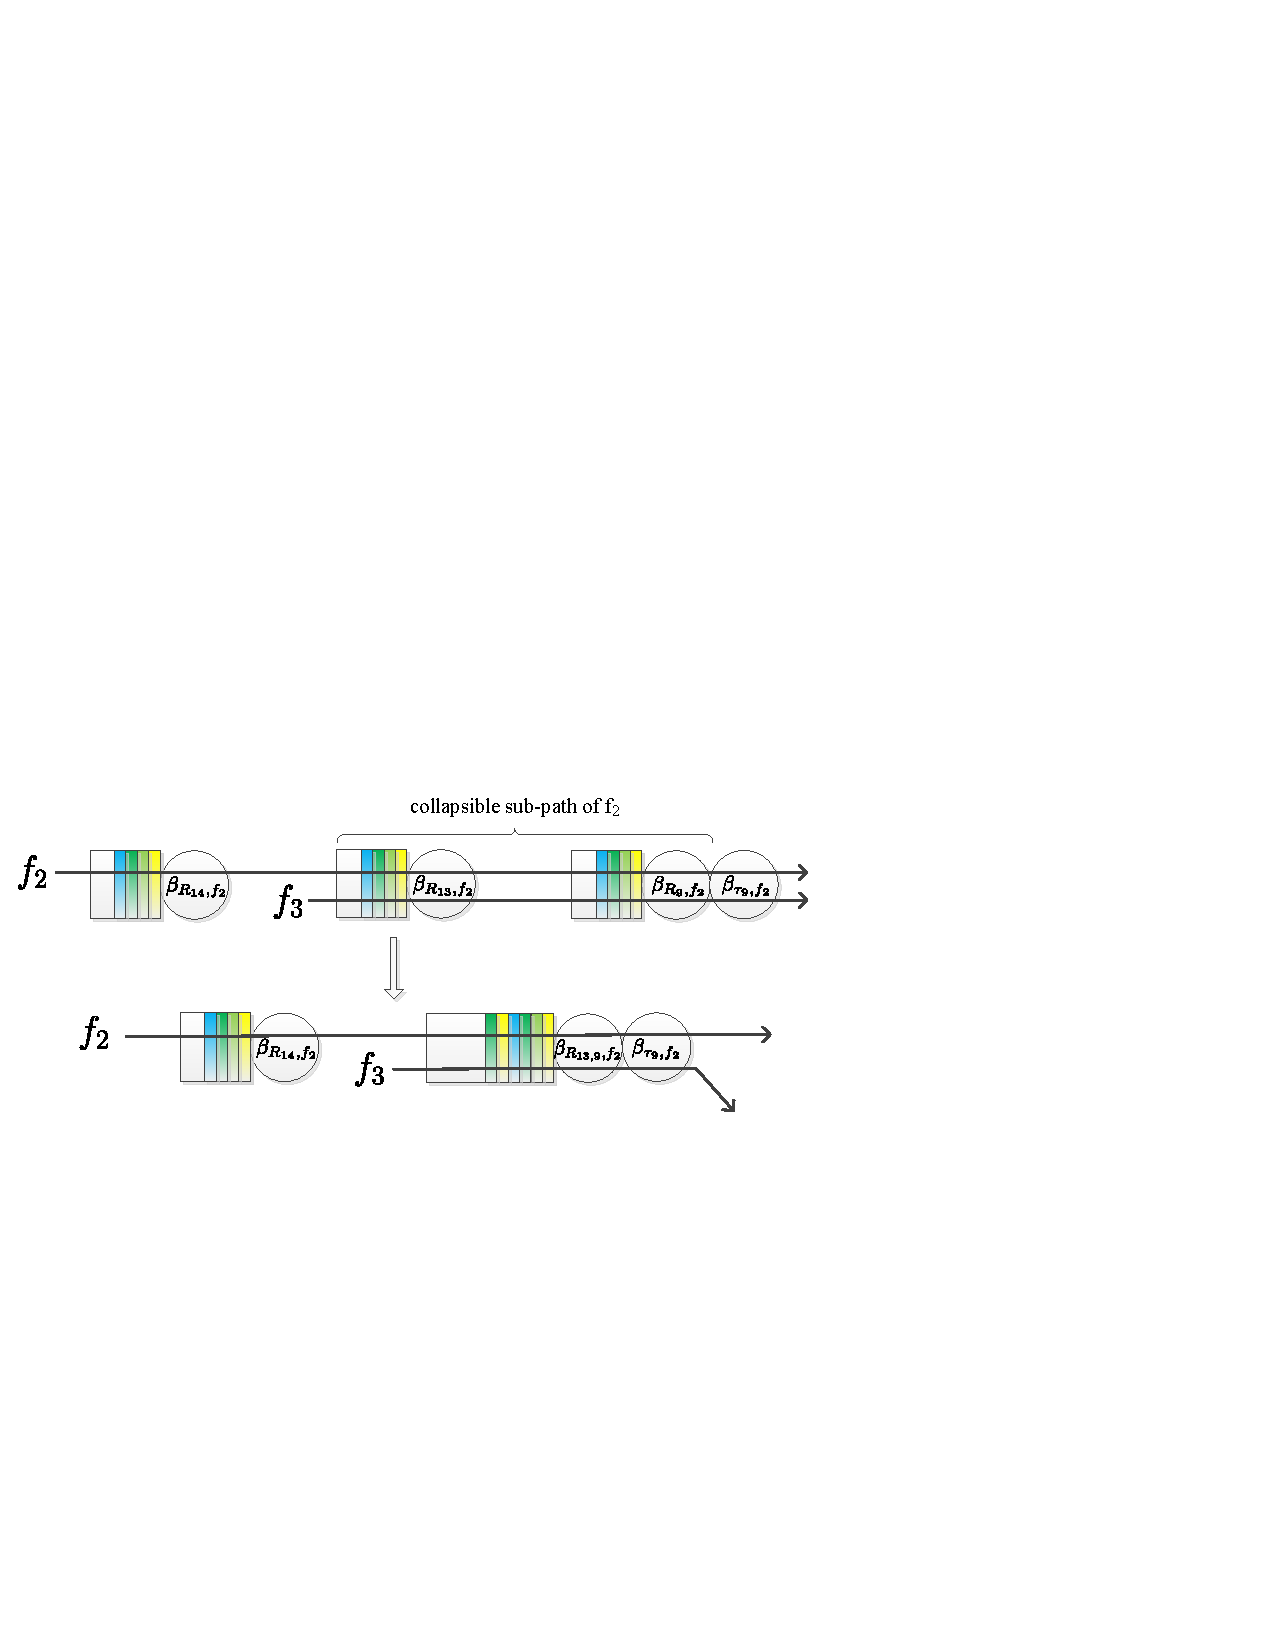
\includegraphics[scale=0.6]{figures/collapse.pdf}\\
  \caption{Collapsible sub-path of $f_2$. Since the flow control between $R_{13}$ and $R_9$ can be neglected, they are replaced by a single virtual router $R_{13,9}$.}\label{collapse}
\end{figure}

\begin{definition}[Collapsible Sub-Path]
A collapsible sub-path of the flow $f_i$ is a router sequence satisfying the following conditions:
\begin{enumerate}
  \item for any router $R_j$ on this sub-path, $M_{R_j,f_i}>1$.
  \item for any two routers on this sub-path, $\Theta_{R_j,f_i}=\Theta_{R_k,f_i}$ and $\Omega_{R_j,f_i}=\Omega_{R_k,f_i}$.
  \item for any router $R_j$ on this sub-path and $\forall f_k\in\Theta_{R_j,f_i}$, $\beta_{R_{j}^{p},f_k}^l\otimes\beta_{\tau_{j},f_k}^l=\beta_{R_{j}^{p},f_k}^l$ and $\beta_{R_{j}^{p},f_k}^u\otimes\beta_{\tau_{j},f_k}^u=\beta_{R_{j}^{p},f_k}^u$ hold unless $R_j$ is the last router on this sub-path.
\end{enumerate}
\end{definition}

The first condition indicates that we should compute the leftover service curve on this sub-path. The second condition ensures that the routers along this sub-path are shared by all the contending flows and the sub-path contains at least two routers. The third condition guarantees that the leftover service curve for low-priority flows can be calculated by first collapsible the sub-path. As implied previously, instead of the router-by-router calculation, we can leverage the concept of CSP and replace all the routers on the collapsible sub-path (denoted as $\mathcal{C}$) with a single virtual router providing service curve $<\otimes_{R_i\in \mathcal{C}}\beta_{R_i^{p},f}^l,\otimes_{R_i\in \mathcal{C}}\beta_{R_i^{p},f}^u>$. For a CSP with $n$ ($n\geq 2$) routers, this method reduces $n-1$ times calculation of arrival curve and leftover service curve. In addition, the accuracy of performance bound can also be improved due to the well-known ``Pay Burst Only Once" phenomenon in the DNC theory \cite{Boudec2001Network}. Each flow may have several CSPs, and the set of all the CSPs of flow $f$ is denoted as $\mathcal{CSP}(f)$. The $\mathcal{CSP}(f)$ can be constructed by scanning the entire path of $f$ once.

\subsection{End-to-End Delay Analysis}\label{e2elatency}
In this subsection, we present the delay analysis algorithm. While constructing the analysis algorithm, the following four issues should be considered carefully: (1) In the fixed-priority flit-level preemptive NoC, only the leftover service curve can be used by the low-priority flows. (2) To simplify the computation and improve the delay bound, we should collapse all the CSPs before computing the leftover service curve for the low-priority flows. (3) Our performance model supports priority-sharing, before computing the leftover service curve for lower priority flows, we must ensure that all the flows with the same priority have been calculated. (4) The computed service curve for flow controller can only be applicable for the specified flow. Keeping these four issues in mind, we propose the end-to-end delay analysis algorithm, as shown in Algorithm \ref{alg:equivalentservicecurve}. This algorithm takes the architecture parameters and flow specification as input, and gives the end-to-end delay of each flow. The architecture parameters specify the network topology graph and buffer size of each VC. The flow specification includes the arrival curve and routine of each flow in $\mathcal{F}$.

\begin{algorithm}
\caption{End-to-End Delay Analysis Algorithm}
\label{alg:equivalentservicecurve}
\begin{algorithmic}[1]
\REQUIRE Architecture parameters and flow specification
\ENSURE Worst-case end-to-end Delay for all the flows
    \FOR {each flow $f_i\in \mathcal{F}$ with priority order}
        \STATE $\beta_{\tau}^l=\delta_0(t)$; $\beta_{\tau}^u=\delta_0(t)$;
        \FOR {each router $R_j\in \mathcal{R}_{i}$ from $end_i$ to $start_i$}
            \IF {$\Theta_{R_j,f_i}\neq \emptyset$}
                \STATE $\beta_{R_j^{p},f_i}^l=\beta_{BW}^l\otimes\beta_{RC}^l\otimes\beta_{VA}^l\otimes\lfloor\frac{\beta_{SA,R_j^{p}}^{l^\prime}}{N_{R_j,f_i}+1}\rfloor\otimes\beta_{ST}^l$;
                \STATE $\beta_{R_j^{p},f_i}^u=\beta_{BW}^u\otimes\beta_{RC}^u\otimes\beta_{VA}^u\otimes\lceil\frac{\beta_{SA,R_j^{p}}^{u^\prime}}{N_{R_j,f_i}+1}\rceil\otimes\beta_{ST}^u$;
            \ELSE
                \STATE $\beta_{R_j^{p},f_i}^l=\beta_{BW}^l\otimes\beta_{RC}^l\otimes\beta_{VA}^l\otimes\beta_{SA,R_j^{p}}^{l^\prime}\otimes\beta_{ST}^l$;
                \STATE $\beta_{R_j^{p},f_i}^u=\beta_{BW}^u\otimes\beta_{RC}^u\otimes\beta_{VA}^u\otimes\beta_{SA,R_j^{p}}^{u^\prime}\otimes\beta_{ST}^u$;
            \ENDIF
            \STATE $\beta^{l}_{\tau_j,f_i}(t)=\beta_{\tau}^l$; $\beta^{u}_{\tau_j,f_i}(t)=\beta_{\tau}^u$;
            \STATE $\beta_{\tau}^l=\overline{\beta^l_{R_j^{p},f_i}\otimes\beta^{l}_{\tau}\otimes\delta_\sigma(t)+B_{R_j^{p},f_i}}$;
            \STATE $\beta_{\tau}^u=\overline{\beta^u_{R_j^{p},f_i}\otimes\beta^{u}_{\tau}\otimes\delta_\sigma(t)+B_{R_j^{p},f_i}}$;
        \ENDFOR
        \STATE $\beta_{\tau_{src},f_i}^l=\beta^l_{\tau}$; $\beta_{\tau_{src},f_i}^u=\beta^u_{\tau}$;
        \STATE $\beta_{f_i}=\beta_{\tau_{src},f_i}^l\otimes (\underset{R_k\in\mathcal{R}_{f_i}}{\otimes}(\beta^l_{R_k,f_i}\otimes\beta^l_{\tau_k,f_i}))$;
        \STATE $Delay(f_i)=H(\alpha^u_{f_i},\beta_{f_i})$;
        \STATE $\beta_{f_i}^l=\beta_{\tau_{src},f_i}^l$; $\beta_{f_i}^u=\beta_{\tau_{src},f_i}^u$;
        \STATE Construct $\mathcal{CSP}(f_i)$;
        \STATE Update $\Theta_{R_j,\cdot}$, $\Omega_{R_j,\cdot}$ and $\mathcal{R}_{\cdot}$ based on $\mathcal{CSP}(f_i)$;
        \FOR {$\forall R_j\in\mathcal{R}_{f_i}$ from $start_i$ to $end_i$}
            \IF {$\Omega_{R_j,f_i}\neq \emptyset$}
                \STATE $\beta^l=\beta^l_{f_i}\otimes\beta_{BW}^l\otimes\beta_{RC}^l\otimes\beta_{VA}^l$;
                \STATE $\beta^u=\beta^u_{f_i}\otimes\beta_{BW}^u\otimes\beta_{RC}^u\otimes\beta_{VA}^u$;
                \STATE $\alpha^l_{R_j,f_i}=\min\{(\alpha^l_{f_i}\oslash\beta^u)\otimes\beta^l,\beta^l\}$;
                \STATE $\alpha^u_{R_j,f_i}=\min\{(\alpha^u_{f_i}\otimes\beta^u)\oslash\beta^l,\beta^u\}$;
                \IF {$\forall f_k\in\Theta_{R_j,f_i}$ have been calculated}
                    \STATE $\alpha^l_{R_j,f_i}=\alpha^l_{R_j,f_i}+\sum_{f_k\in\Theta_{R_j,f_i}}\alpha^l_{R_j,f_k}$;
                    \STATE $\alpha^u_{R_j,f_i}=\alpha^u_{R_j,f_i}+\sum_{f_k\in\Theta_{R_j,f_i}}\alpha^u_{R_j,f_k}$;
                    \STATE $\beta^{l^\prime}_{SA,R_j^{p}}=(\beta^{l^\prime}_{SA,R_j^{p}}-\alpha^u_{R_j,f_i})\bar{\otimes}0$;
                    \STATE $\beta^{u^\prime}_{SA,R_j^{p}}=\max\{(\beta^{u^\prime}_{SA,R_j^{p}}-\alpha^l_{R_j,f_i})\bar{\oslash}0,0\}$;
                \ENDIF
            \ENDIF
            \STATE $\beta_{f_i}^l=\beta_{f_i}^l\otimes\beta^l_{R_j^{p},f_i}$; $\beta_{f_i}^u=\beta_{f_i}^u\otimes\beta^u_{R_j^{p},f_i}$;
        \ENDFOR
    \ENDFOR
\end{algorithmic}
\end{algorithm}

In this algorithm, the arrival curve of flow $f_i$ at the source NI and router $R_j$ are denoted as $<\alpha_{f_i}^l,\alpha_{f_i}^u>$ and $<\alpha_{R_j,f_i}^l,\alpha_{R_j,f_i}^u>$, respectively. The leftover service curve of switch allocator at output port $p$ is represented as $<\beta_{SA,R_j^{p}}^{l^\prime},\beta_{SA,R_j^{p}}^{u^\prime}>$ (Initially, let $\beta_{SA,R_j^{p}}^{l^\prime}=\beta_{SA,R_j^{p}}^{l}$ and $\beta_{SA,R_j^{p}}^{u^\prime}=\beta_{SA,R_j^{p}}^{u}$). To address the four issues mentioned above, our algorithm computes the delay bound from high-priority flows to low-priority flows. For each iteration, it performs the following four steps in sequence: (1) Calculating the service curves provided by the routers (lines 4-10) and flow controllers (lines 11-12) along the path. (2) Identifying and collapsing all the CSPs on the path of a flow (line 14). (3) Computing the worst-case end-to-end delay of the flow (line 15). (4) Calculating the leftover service curve at each router for low-priority flows when all the service curves of high-priority flows have been calculated (lines 16-32). The overall algorithm has two-level embedded loops, and the computation complexity for this algorithm is $O(HN)$, where $N$ and $H$ is the number of flows and the hop count of each flow. This complexity is pseudo-polynomial due to the numerical computation of convolution. This algorithm can be easily integrated into the RTC toolbox \cite{rtc} to compute the end-to-end delay bound automatically.

\subsection{Buffer Sizing}\label{bufferopt}
The priority-aware wormhole-switched NoC \cite{Shi:2008:RCA:1397757.1397996} requires the same amount of VC as the priorities to prevent priority inversion \cite{707545}, which refers to the blocking of high-priority flows when the low-priority flows occupy all the VCs. To reduce the buffer area and power consumption, priority sharing \cite{5161497} and buffer optimization \cite{189} techniques have been proposed. However, two backlog bounds derived in \cite{189} are the minimum buffer size that does not trigger the flow control, which can be further reduced as long as the deadline constraint is not being violated. Suppose the applications have been mapped onto the NoC, and each flow $f_i$ has been assigned to their corresponding priority $P_i$ and deadline $D_i$. Following the same notation as Algorithm 1, we propose the buffer sizing algorithm to further reduce the buffer size, as shown in Algorithm \ref{alg:bufopt}. It tries to reduce the buffer size for each flow from high-priority to low-priority gradually. For each iteration, it performs the following four steps: (1) Calculating the service curves provided by the routers (lines 3-9). (2) Calculate the minimum buffer size that can avoid flow control for each router (lines 10-13). (3) Reduce the initial buffer size gradually as long as the constraint of deadline is not being violated (lines 15-26). (4) Calculating the leftover service curve at each router for low-priority flows (lines 27-43). This algorithm can be implemented in RTC toolbox \cite{rtc} to optimize the buffer size automatically. The entire computation complexity is $O(HN)$, where $N$ and $H$ are the number of flows and the hop count of each flow. This complexity is also pseudo-polynomial due to the numerical computation of convolution.
\begin{algorithm}
\caption{Buffer Sizing Algorithm}
\label{alg:bufopt}
\begin{algorithmic}[1]
\REQUIRE Architecture parameters and flow specification
\ENSURE Optimized buffer size
    \FOR {each flow $f_i\in \mathcal{F}$ with priority order}
        \FOR {each router $R_j\in \mathcal{R}_{i}$}
            \IF {$\Theta_{R_j,f_i}\neq \emptyset$}
                \STATE $\beta_{R_j^{p},f_i}^l=\beta_{BW}^l\otimes\beta_{RC}^l\otimes\beta_{VA}^l\otimes\lfloor\frac{\beta_{SA,R_j^{p}}^{l^\prime}}{N_{R_j,f_i}+1}\rfloor\otimes\beta_{ST}^l$;
                \STATE $\beta_{R_j^{p},f_i}^u=\beta_{BW}^u\otimes\beta_{RC}^u\otimes\beta_{VA}^u\otimes\lceil\frac{\beta_{SA,R_j^{p}}^{u^\prime}}{N_{R_j,f_i}+1}\rceil\otimes\beta_{ST}^u$;
            \ELSE
                \STATE $\beta_{R_j^{p},f_i}^l=\beta_{BW}^l\otimes\beta_{RC}^l\otimes\beta_{VA}^l\otimes\beta_{SA,R_j^{p}}^{l^\prime}\otimes\beta_{ST}^l$;
                \STATE $\beta_{R_j^{p},f_i}^u=\beta_{BW}^u\otimes\beta_{RC}^u\otimes\beta_{VA}^u\otimes\beta_{SA,R_j^{p}}^{u^\prime}\otimes\beta_{ST}^u$;
            \ENDIF
            \STATE $B^l=\inf\{B|\beta_{R_j^{p},f_i}^l\otimes\overline{\beta_{R_j^{p},f_i}^l\otimes\delta_\sigma(t)+B}\geq\beta_{R_j^{p},f_i}^l\}$;
            \STATE $B^u=\inf\{B|\beta_{R_j^{p},f_i}^u\otimes\overline{\beta_{R_j^{p},f_i}^u\otimes\delta_\sigma(t)+B}\geq\beta_{R_j^{p},f_i}^u\}$;
            \STATE $B_{R_j^{p},f_i}=\max\{B^l,B^u\}$;
            \STATE $\beta_{\tau_j,f_i}^l=\delta_0(t)$; $\beta_{\tau_j,f_i}^u=\delta_0(t)$;
        \ENDFOR
        \STATE $\beta_{\tau_{src},f_i}^l=\beta^l_{\tau}$; $\beta_{\tau_{src},f_i}^u=\beta^u_{\tau}$;
        \FOR {each router $R_j\in \mathcal{R}_{i}$ from $end_i$ to $start_i$}
            \STATE $\beta_{f_i}=\beta_{\tau_{src},f_i}^l\otimes\underset{R_k\in\mathcal{R}_{f_i}}{\otimes}(\beta^l_{R_k^p,f_i}\otimes\beta^l_{\tau_k,f_i})$;
            \STATE $Delay(f_i)=H(\alpha^u_{f_i},\beta_{f_i})$;
            \WHILE {$Delay(f_i)\leq D_i$ and $B_{R_j^p,f_i}>1$}
                \STATE $B_{R_j^p,f_i}=B_{R_j^p,f_i}-1$;
                \STATE Update $\beta_{\tau_k,f_i}^l$ for all $R_{k}$ from $R_j$ to $start_i$;
                \STATE $\beta_{f_i}=\beta_{\tau_{src},f_i}^l\otimes\underset{R_k\in\mathcal{R}_{f_i}}{\otimes}(\beta^l_{R_k^p,f_i}\otimes\beta^l_{\tau_k,f_i})$;
                \STATE $Delay(f_i)=H(\alpha^u_{f_i},\beta_{f_i})$;
            \ENDWHILE
            \IF {$Delay(f_i)>D_i$}
                \STATE $B_{R_j^p,f_i}=B_{R_j^p,f_i}+1$;
                \STATE Update $<\beta_{\tau_j,f_i}^l,\beta_{\tau_j,f_i}^u>$;
            \ENDIF
        \ENDFOR
        \STATE $\beta_{f_i}^l=\beta_{\tau_{src},f_i}^l$; $\beta_{f_i}^u=\beta_{\tau_{src},f_i}^u$;
        \FOR {$\forall R_j\in\mathcal{R}_{f_i}$ from $start_i$ to $end_i$}
            \IF {$\Omega_{R_j,f_i}\neq \emptyset$}
                \STATE $\beta^l=\beta^l_{f_i}\otimes\beta_{BW}^l\otimes\beta_{RC}^l\otimes\beta_{VA}^l$;
                \STATE $\beta^u=\beta^u_{f_i}\otimes\beta_{BW}^u\otimes\beta_{RC}^u\otimes\beta_{VA}^u$;
                \STATE $\alpha^l_{R_j,f_i}=\min\{(\alpha^l_{f_i}\oslash\beta^u)\otimes\beta^l,\beta^l\}$;
                \STATE $\alpha^u_{R_j,f_i}=\min\{(\alpha^u_{f_i}\otimes\beta^u)\oslash\beta^l,\beta^u\}$;
                \IF {$\forall f_k\in\Theta_{R_j,f_i}$ have been calculated}
                    \STATE $\alpha^l_{R_j,f_i}=\alpha^l_{R_j,f_i}+\sum_{f_k\in\Theta_{R_j,f_i}}\alpha^l_{R_j,f_k}$;
                    \STATE $\alpha^u_{R_j,f_i}=\alpha^u_{R_j,f_i}+\sum_{f_k\in\Theta_{R_j,f_i}}\alpha^u_{R_j,f_k}$;
                    \STATE $\beta^{l^\prime}_{SA,R_j^{p}}=(\beta^{l^\prime}_{SA,R_j^{p}}-\alpha^u_{R_j,f_i})\bar{\otimes}0$;
                    \STATE $\beta^{u^\prime}_{SA,R_j^{p}}=\max\{(\beta^{u^\prime}_{SA,R_j^{p}}-\alpha^l_{R_j,f_i})\bar{\oslash}0,0\}$;
                \ENDIF
            \ENDIF
            \STATE $\beta_{f_i}^l=\beta_{f_i}^l\otimes\beta^l_{R_j^{p},f_i}$; $\beta_{f_i}^u=\beta_{f_i}^u\otimes\beta^u_{R_j^{p},f_i}$;
        \ENDFOR
    \ENDFOR
\end{algorithmic}
\end{algorithm}

A significant difference with Algorithm 1 is that, this algorithm does not identify and collapse all the CSPs for each flow, because the reduction of buffer size introduces flow control between adjacent routers, which prevents the flits progressing in the network and leads to a larger end-to-end delay. The amount of cycles that a packet can be stalled in the network without violating the deadline is defined as `slack'. Our buffer sizing algorithm can reduce the buffer size iteratively as long as slack is greater than zero, which can be used to reduce the router area and power consumption. However, it is significantly different from the DNC based slack optimization in \cite{6560630}. In \cite{6560630}, the energy optimization is achieved by adjusting the voltage, frequency and link bandwidth of on-chip routers for the fixed configuration and deadline. In contrast, our method tries to optimize the buffer size under the deadline constraint, and the buffer reduction directly leads to the area and power saving. In addition, our algorithm can be used in conjunction with the priority sharing techniques \cite{5161497} to optimize the buffer size of priority-aware wormhole-switched NoC.

\section{Experiments}\label{experiments}
In this section, we validate the correctness and tightness of our performance model by comparison with other analytical methods and simulation. Several analytical methods exist for the delay analysis of priority-aware NoC, examples include contention tree model \cite{LuJS05}, lumped link model \cite{707545}, dependency graph model \cite{708526}, FLA \cite{Shi:2008:RCA:1397757.1397996}, LLA \cite{73} and DNC \cite{Qian489900}, etc. There are also extensive research on the buffer sizing of the priority-aware NoC, representative works include shaping delay analysis \cite{Manolache:2006:BSO:1131481.1131683} and LLBA \cite{189}. Among all these analytical methods, LLA \cite{73}\cite{189} and DNC \cite{Qian489900} based model outperform the others when the tightness of delay and backlog bound are considered. Thus, we will only perform the comparison with LLA and DNC, as presented in subsection \ref{llacmp} and subsection \ref{dnccmp}, respectively.

\subsection{Comparison with Link Level Analysis}\label{llacmp}
The network topology and flows are shown in Fig. \ref{topology}. There are four flows (i.e. $f_1$, $f_2$, $f_3$ and $f_4$) in the network, with different priority $P_4>P_1>P_2>P_3$. Suppose the packet length of flow $f_i$ is $F_i$ (in flits), and the injection period is $I_i$. We perform the comparison on a set of periodical traffic due to the restriction of LLA method \cite{73}\cite{189}, and the traffic jitter for all the flows are set to be zero. To ease the analysis, LLA supposes the number of bits in a flit is the same as the physical channel width, and the latency of a flit traverses a router is one cycle. To compare with LLA, our model for the standard five stages wormhole router should be specialized to a single-cycle router, this is achieved by letting the service curve of BW, RC, VA and ST stage be a burst delay function $\delta_0(t)$. Under this condition, the service curve of the entire router is the same as the service curve provided by the SA stage, which is $<\beta_{SA,R_i^p}^l,\beta_{SA,R_i^p}^u>$. In addition, the LLA method does not consider the self-blocking caused by flow control. Thus, we set the credit feedback delay $\sigma=0$ cycle in our model for a fair comparison. Next, we compare the end-to-end delay and buffer requirement computed with LLA and our model.

\subsubsection{End-to-End Delay}
For this scenario, we suppose the VC buffer is large enough so that we can neglect the back-pressure caused by flow control and directly apply LLA for the delay analysis. Suppose all the flows have the same injection period $I_i$ and packet length $F_i$, we examine the end-to-end delay of the four flows in Fig. \ref{topology} under different packet length $F_i$ and injection period $I_i$, the calculated result is shown in Table \ref{LLAvsRTC}. The RTC result is obtained by collapsing the CSP of $f_2$ (i.e. $R_{13}$ and $R_{9}$). Each quaternion in the table corresponds to the worst-case delay of $f_1$, $f_2$, $f_3$ and $f_4$ (in cycles). The blank items corresponding to LLA columns indicate that the worst-case delay of a flow is greater than its injection period, which cannot be analyzed with LLA \cite{73}\cite{189}, and the blank items corresponding to RTC columns indicate that the network is unstable because the injection rate exceeds the processing capability of the network. As shown in Table \ref{LLAvsRTC}, the RTC method is applicable to these scenarios which can not be analyzed by LLA. In addition, we also observed from the table that the RTC result is as tight as that of LLA except for the scenarios that the worst-case delay of a flow is close to the injection period, e.g. $F_i=1$, $I_i=6$ in Table \ref{LLAvsRTC}. The root cause of these exceptions is that RTC theory we used in this paper is a counter-based algebra approach, which ignores some state information of the entire network. Although the counter-based approach, e.g. timed automata \cite{Fersman2006301} and event count automata \cite{Chakraborty:2005:ECA:1106608.1106642}, can be applied to improve our results, they will lead to higher computation complexity and state space explosion.
\begin{table}[htbp]
\centering
\caption{\label{LLAvsRTC}Delay comparison with link level analysis}
\begin{tabular}{|c|c|c|c|c|c|c|}
\hline
\multirow{3}{*}{$I_i$}  & \multicolumn{2}{|c|}{$F_i=1$} & \multicolumn{2}{|c|}{$F_i=2$}    &   \multicolumn{2}{|c|}{$F_i=4$} \\
\cline{2-7}
& RTC & LLA & RTC & LLA &   RTC &   LLA\\
\hline
$3$ &   7,7,8,4 &   --- &   --- &   ---   &      --- &   --- \\
\hline
$4$ &   6,6,6,4 &   --- &   --- &   ---   &      --- &   --- \\
\hline
$5$ &   6,6,6,4 &   --- &   9,10,12,5 &   ---   &      --- &   --- \\
\hline
$6$ &   5,6,6,4 &   5,6,5,4 &   9,8,9,5 &   ---   &      --- &   --- \\
\hline
$7$ &   5,6,5,4 &   5,6,5,4 &   9,8,9,5 &   --- &      --- &   --- \\
\hline
$8$ &   5,6,5,4 &   5,6,5,4 &   7,8,9,5 &   7,8,7,5 &      --- &   --- \\
\hline
$9$ &   5,6,5,4 &   5,6,5,4 &   7,8,9,5 &   7,8,7,5 &   15,16,19,7 &   --- \\
\hline
$10$    &   5,6,5,4 &   5,6,5,4 &   7,8,7,5 &   7,8,7,5 &   15,12,15,7  &   ---\\
\hline
$11$    &   5,6,5,4 &   5,6,5,4 &   7,8,7,5 &   7,8,7,5 &   15,12,15,7  &   ---\\
\hline
$12$    &   5,6,5,4 &   5,6,5,4 &   7,8,7,5 &   7,8,7,5 &   11,12,15,7  &   ---\\
\hline
$13$    &   5,6,5,4 &   5,6,5,4 &   7,8,7,5 &   7,8,7,5 &   11,12,15,7  &   ---\\
\hline
$14$    &   5,6,5,4 &   5,6,5,4 &   7,8,7,5 &   7,8,7,5 &   11,12,15,7  &   ---\\
\hline
$15$    &   5,6,5,4 &   5,6,5,4 &   7,8,7,5 &   7,8,7,5 &   11,12,15,7  &   11,12,11,7\\
\hline
$16$    &   5,6,5,4 &   5,6,5,4 &   7,8,7,5 &   7,8,7,5 &   11,12,11,7  &   11,12,11,7\\
\hline
$17$    &   5,6,5,4 &   5,6,5,4 &   7,8,7,5 &   7,8,7,5 &   11,12,11,7  &   11,12,11,7\\
\hline
\end{tabular}
\end{table}

\subsubsection{Buffer Sizing}
The LLBA method \cite{189} can only give the required buffer size at each VC to prevent flow control, because the flow control can lead to the chain blocking in the network, which complicates the analysis with LLBA. Our RTC-based performance model can model the flow control behavior in a natural way, because we abstract the flow control mechanism with the wide-sense service curve. By taking the flow control into consideration, our buffer sizing algorithm can be utilized to reduce the buffer size calculated with LLBA method further as long as the deadline constraint is not violated. We take a simple example to demonstrate the strength of our method. Suppose all the flows have the same packet injection period $I_i=20$ cycles and packet length $F_i=4$ flits ($i=1,2,3,4$), we can get the end-to-end delay with LLA method for the four flows, which are (11,12,11,7) cycles. We can also get the buffer size reserved at each router for the four flows with LLBA method, which are $(1,1,1,4)$, $(4,1,1,1,1)$, $(4,4,1,1)$ and $(1,1,1,1)$, respectively. For the same configuration, if we change the deadline constraint from 15 cycles to 27 cycles, the buffer required for each flow can be further reduced with our buffer sizing algorithm, as shown in Table \ref{LLBAvsRTC}. Take the deadline $D_i=27$ as an example, the calculated buffer size is $17/29\approx58.62$\% smaller than the total buffer size calculated with the LLBA method.
\begin{table}[htbp]
\centering
\caption{\label{LLBAvsRTC}buffer requirement computed with RTC model}
\begin{tabular}{|c|c|c|c|c|c|c|}
\hline
Deadline  & $f_1$  &   $f_2$   &   $f_3$   &   $f_4$   &   Total\\
\hline
(15,15,15,15)   &   (1,1,1,2)   &   (2,1,1,1,1) &   (4,4,1,1)   &   (1,1,1,1)   &   25\\
\hline
(17,17,17,17)   &   (1,1,1,2)   &   (2,1,1,1,1) &   (3,3,1,1)   &   (1,1,1,1)   &   23\\
\hline
(19,19,19,19)   &   (1,1,1,2)   &   (2,1,1,1,1) &   (2,2,1,1)   &   (1,1,1,1)   &   22\\
\hline
(21,21,21,21)   &   (1,1,1,2)   &   (1,1,1,1,1) &   (2,2,1,1)   &   (1,1,1,1)   &   20\\
\hline
(23,23,23,23)   &   (1,1,1,1)   &   (1,1,1,1,1) &   (2,2,1,1)   &   (1,1,1,1)   &   19\\
\hline
(25,25,25,25)   &   (1,1,1,1)   &   (1,1,1,1,1) &   (2,2,1,1)   &   (1,1,1,1)   &   19\\
\hline
(27,27,27,27)   &   (1,1,1,1)   &   (1,1,1,1,1) &   (1,1,1,1)   &   (1,1,1,1)   &   17\\
\hline
\end{tabular}
\end{table}

\subsection{Comparison with Network Calculus}\label{dnccmp}
In this subsection, we present the numerical results to demonstrate the improvement of our method over DNC method proposed in \cite{Qian489900}. We use the periodical traffic as an example to make the comparison. Denote by $I_i$ the injection period, $F_i$ the packet length, the arrival curve can be easily obtained according to the method introduced in subsection \ref{traffic}. Suppose the priority of each flow in Fig. \ref{topology} satisfies $P_4>P_1>P_2>P_3$, the buffer depth at each router $B=15$ flits, credit feedback delay $\sigma=0$ cycle. Define injection rate $V_i=F_i/I_i$, we change $V_i$ ($i=1,2,3,4$) from $1/3$ to $1/6$ flits/cycle and packet length from $1$ to $8$ flits, the end-to-end delay of flow $f_3$ calculated with the DNC-based and our method are plotted in Fig. \ref{comparison}. By comparison, we find that our method can derive a much tighter delay bound than the DNC method proposed in \cite{Qian489900}. The root cause for this improvement lies in the fact that our method utilizes the upper service curve to limit the output upper arrival curve, and further leads to a tighter lower service curve for the low-priority flows. To demonstrate this, let $F_i=8$ flits and $V_i=1/6$ flits/cycle, we plot the service curve for flow $f_3$ calculated with the DNC and RTC in Fig. \ref{loose}. The service curve is calculated with RTC toolbox. From Fig. \ref{loose}, we find that the calculated service curve with DNC is indeed looser than the service curve calculated with our method. Since the delay bound is the maximal horizontal deviation between upper arrival curve and lower service curve in this figure, this looser service curve will finally lead to a looser end-to-end delay bound.
\begin{figure}
  \centering
  % Requires \usepackage{graphicx}
  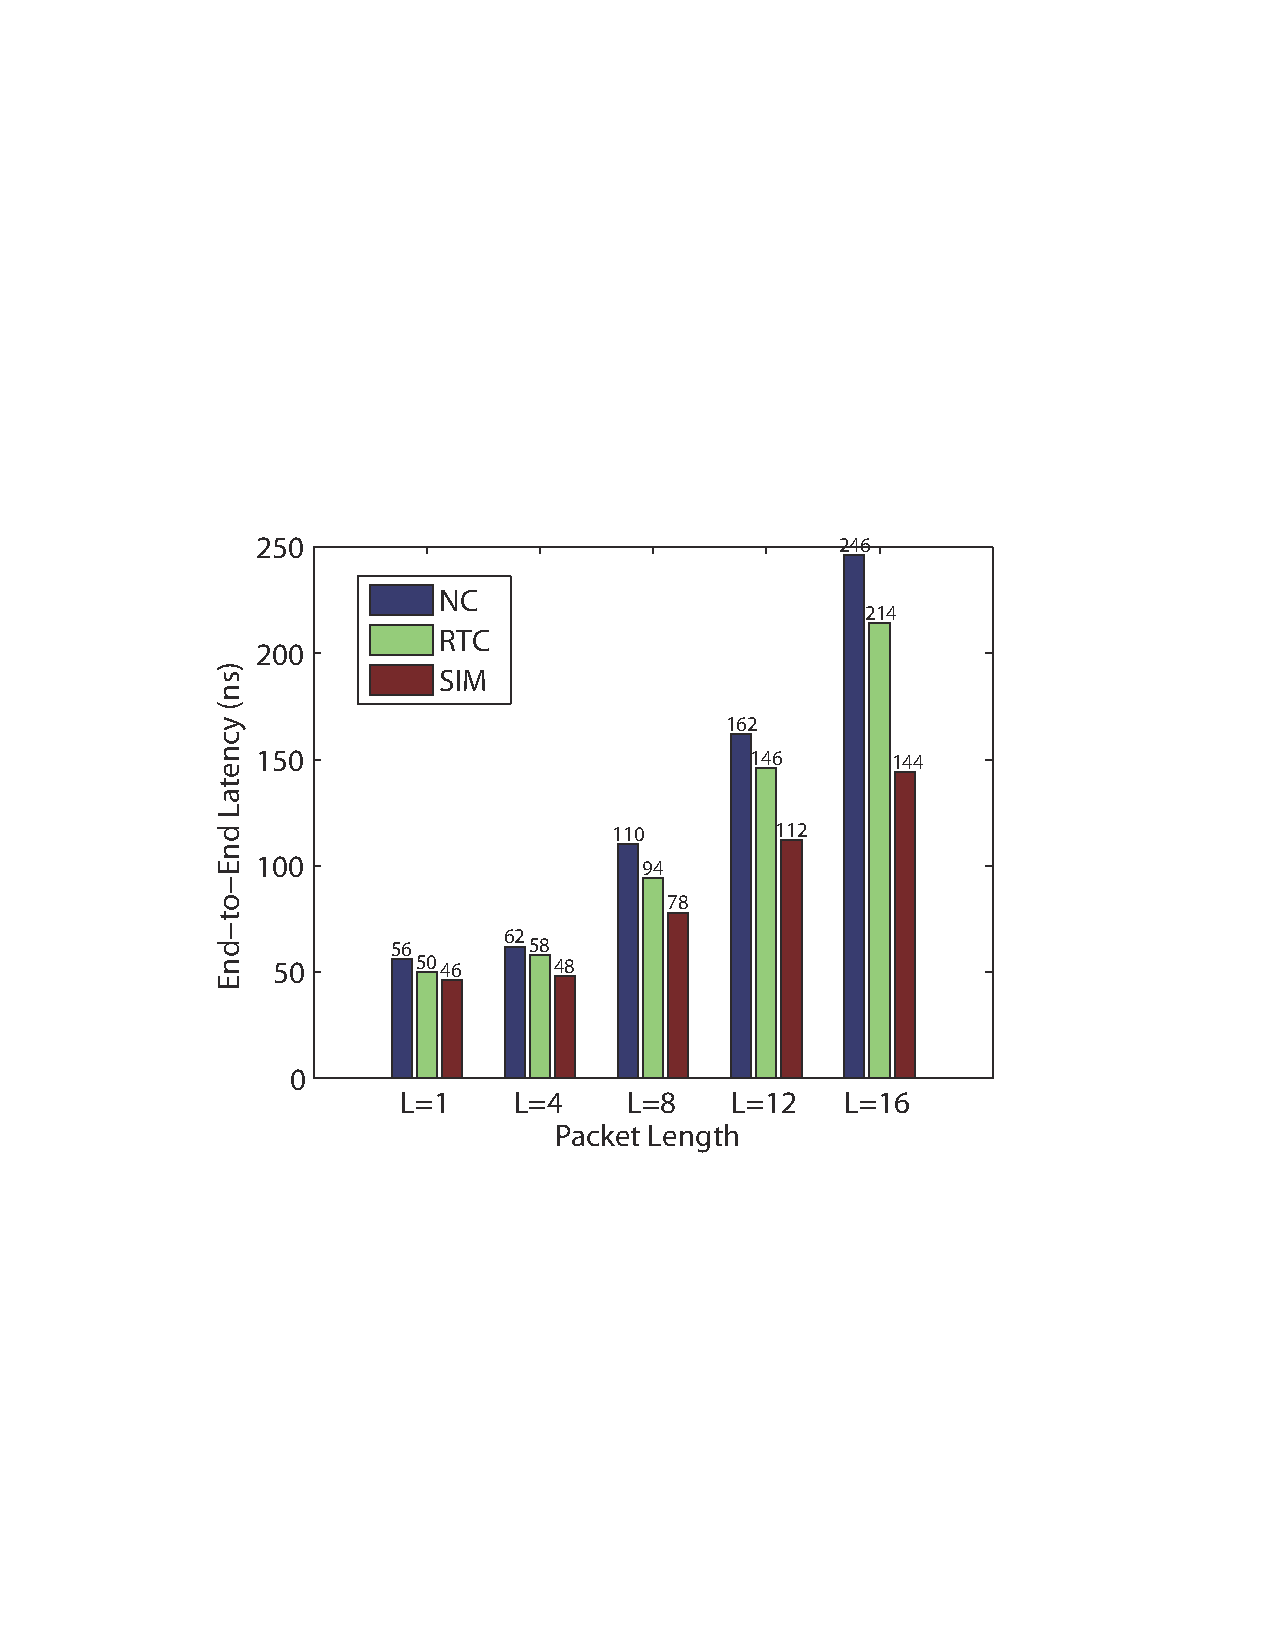
\includegraphics[scale=0.65]{figures/comparison.pdf}\\
  \caption{Comparison with network calculus}\label{comparison}
\end{figure}
\begin{figure}
  \centering
  % Requires \usepackage{graphicx}
  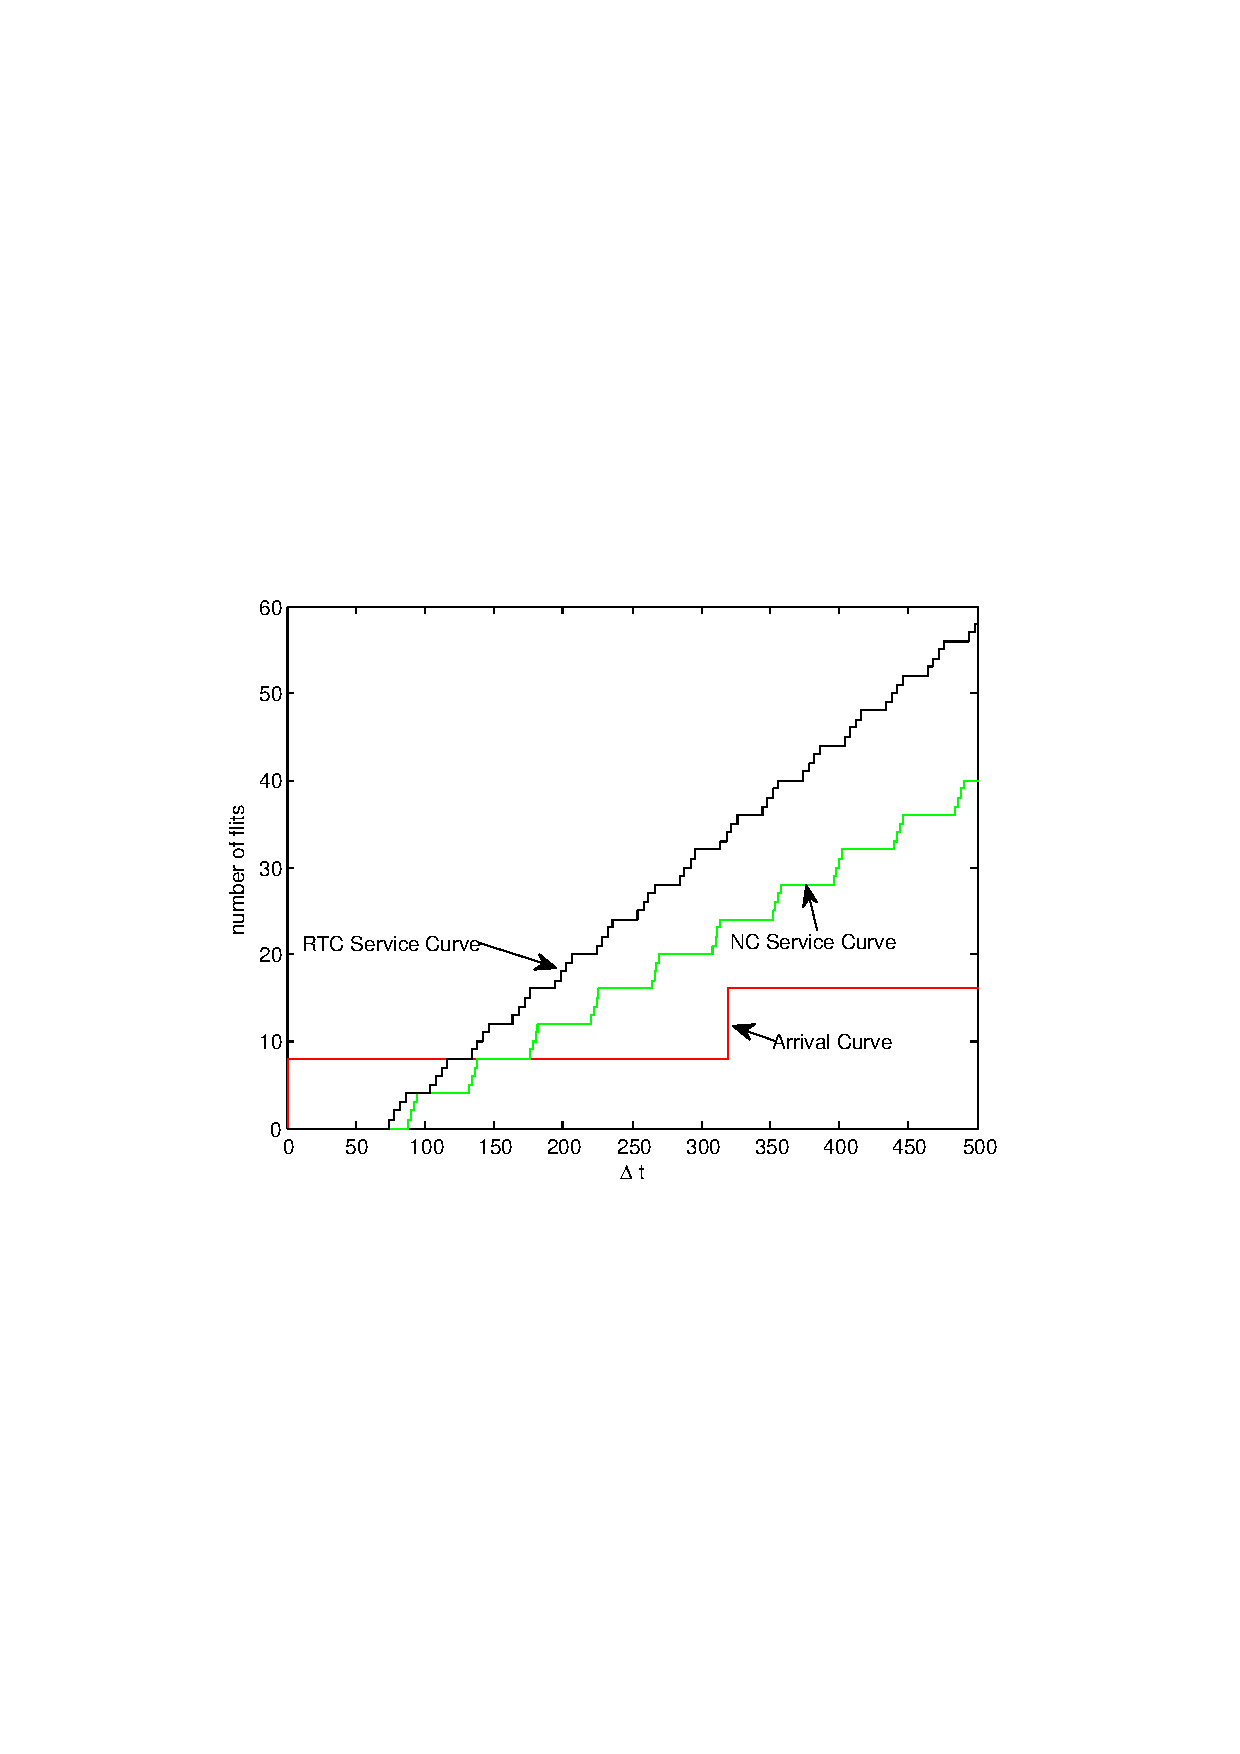
\includegraphics[scale=0.65]{figures/loose.pdf}\\
  \caption{Service curve derived from RTC and DNC}\label{loose}
\end{figure}

The comparison results in Fig. \ref{comparison} also exhibits two special data points calculated with our method need to be explained. For the given injection rate $V_i=1/6$ ($1/5$) flits/cycle, when we increase the packet length $F_i=7$ to $F_i=8$ flits, the worst-case delay calculated with our method decreases from 47 to 43 (49 to 47) cycles. To explain this phenomenon, for the given injection rate $V_i=1/6$ flits/cycle, we plot the upper arrival curve and lower service curve of flow $f_3$ in Fig. \ref{reason} for both $F_i=7$ and $F_i=8$ scenarios. As indicated in this figure, when $F_i=8$ flits, the lower service curve for $f_3$ is greater than that of $F_i=7$ flits between the time interval $[41,51]$, which leads to a smaller delay bound than $F_i=7$.
\begin{figure}
  \centering
  % Requires \usepackage{graphicx}
  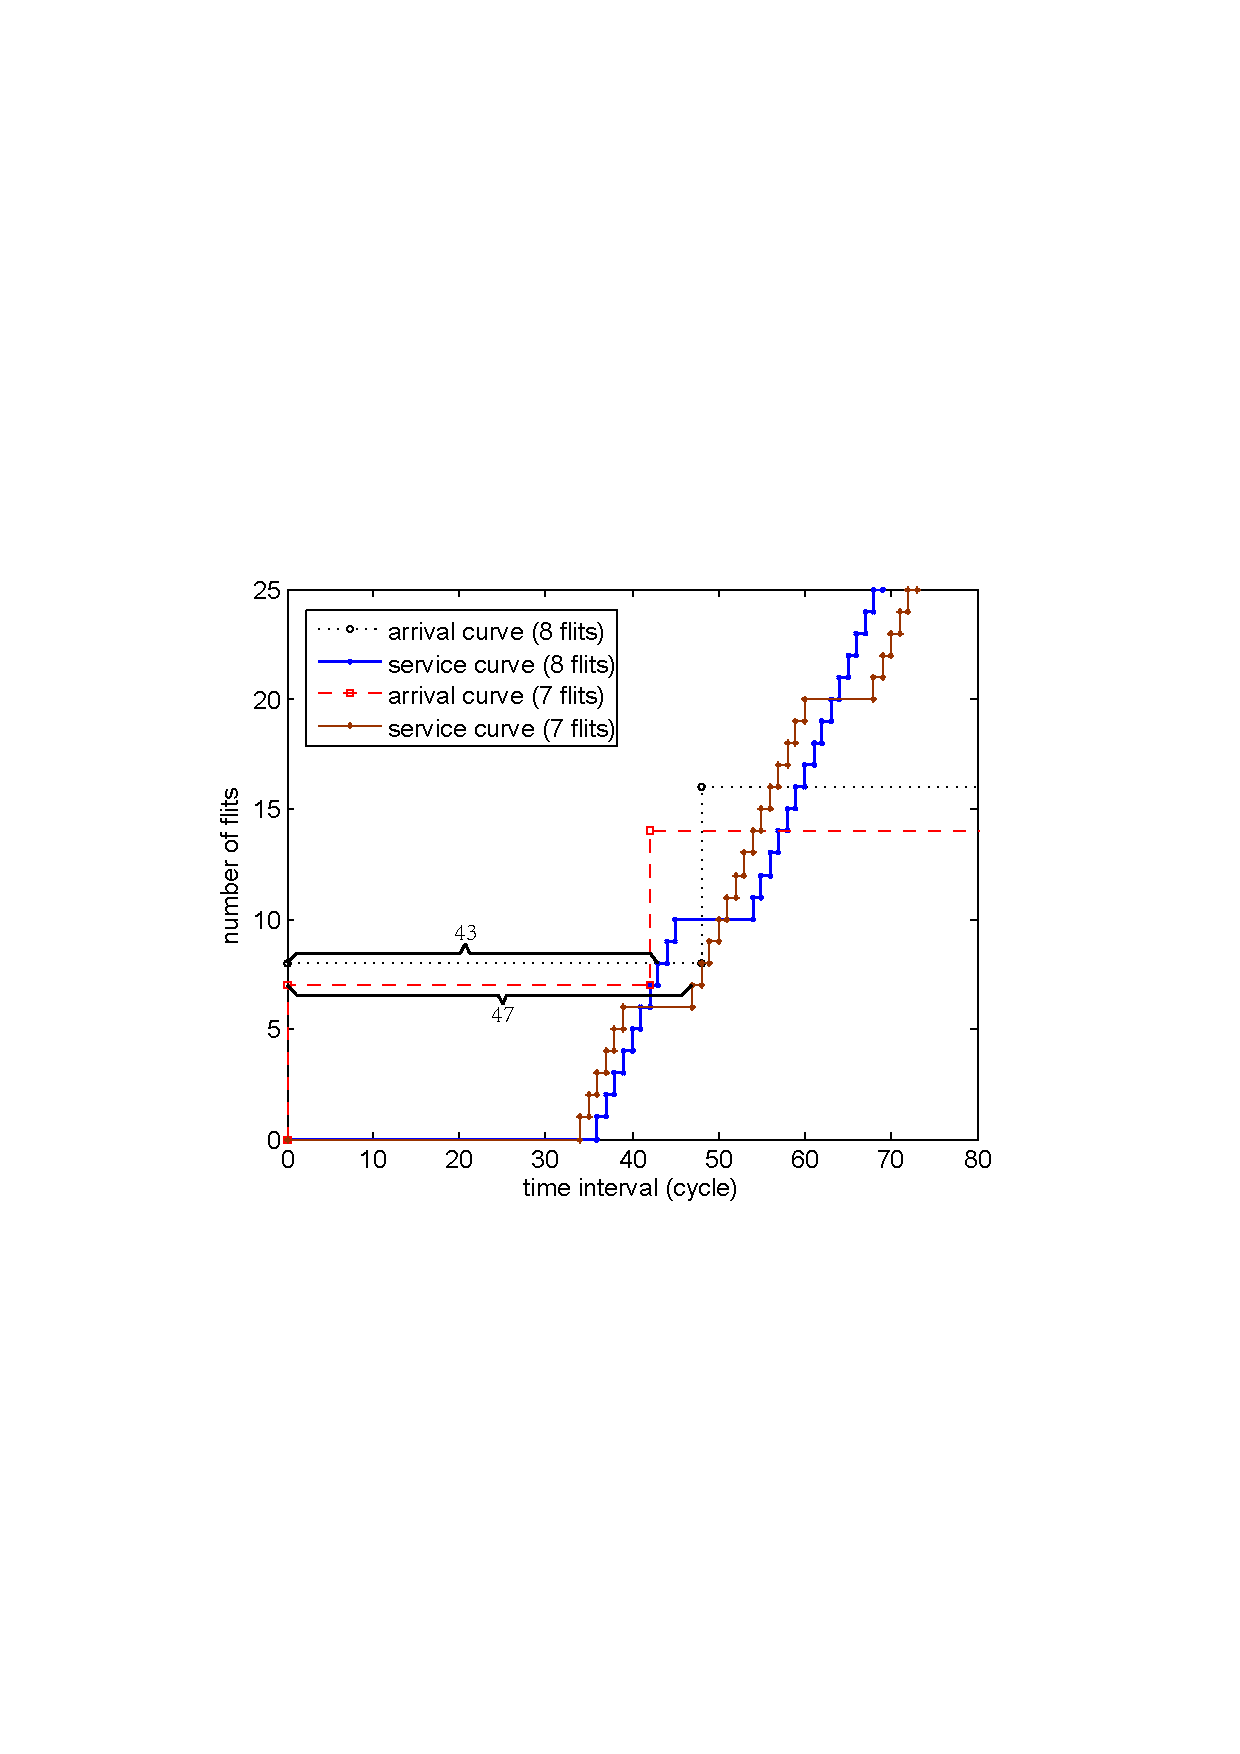
\includegraphics[scale=0.63]{figures/reason.pdf}\\
  \caption{Delay Comparison between $F_i=7$ and $F_i=8$}\label{reason}
\end{figure}

\subsection{Comparison with Simulation}
The correctness of our delay analysis algorithm and buffer sizing algorithm is verified by simulation. We modified the switch allocator of a modular open source NoC simulator, Heterogenous Networks-on-Chip (HNoCs) \cite{6404157}, to support fixed-priority scheduling, and collect the maximum end-to-end packet delay at each destination IP core. For the same injection rate $V_i=1/6$ flits/cycle, we change the packet length from two flits to nine flits, and collect the end-to-end delay of the four flows in Fig. \ref{topology} obtained by simulation and our method. The comparison results are shown in Fig. \ref{rtcvssim}, to prevent the results of flow $f_2$ from shading the results of $f_3$, we exchange the order of $f_3$ and $f_4$ in this figure. As indicated in the comparison, for the given configuration, delay calculated with our method is indeed an upper bound of the simulation results, which verifies the correctness of our methods. In addition, we also found that, the delay bound of high-priority flows (e.g. $f_1$ and $f_4$) is tighter than that of low-priority flows.
\begin{figure}
  \centering
  % Requires \usepackage{graphicx}
  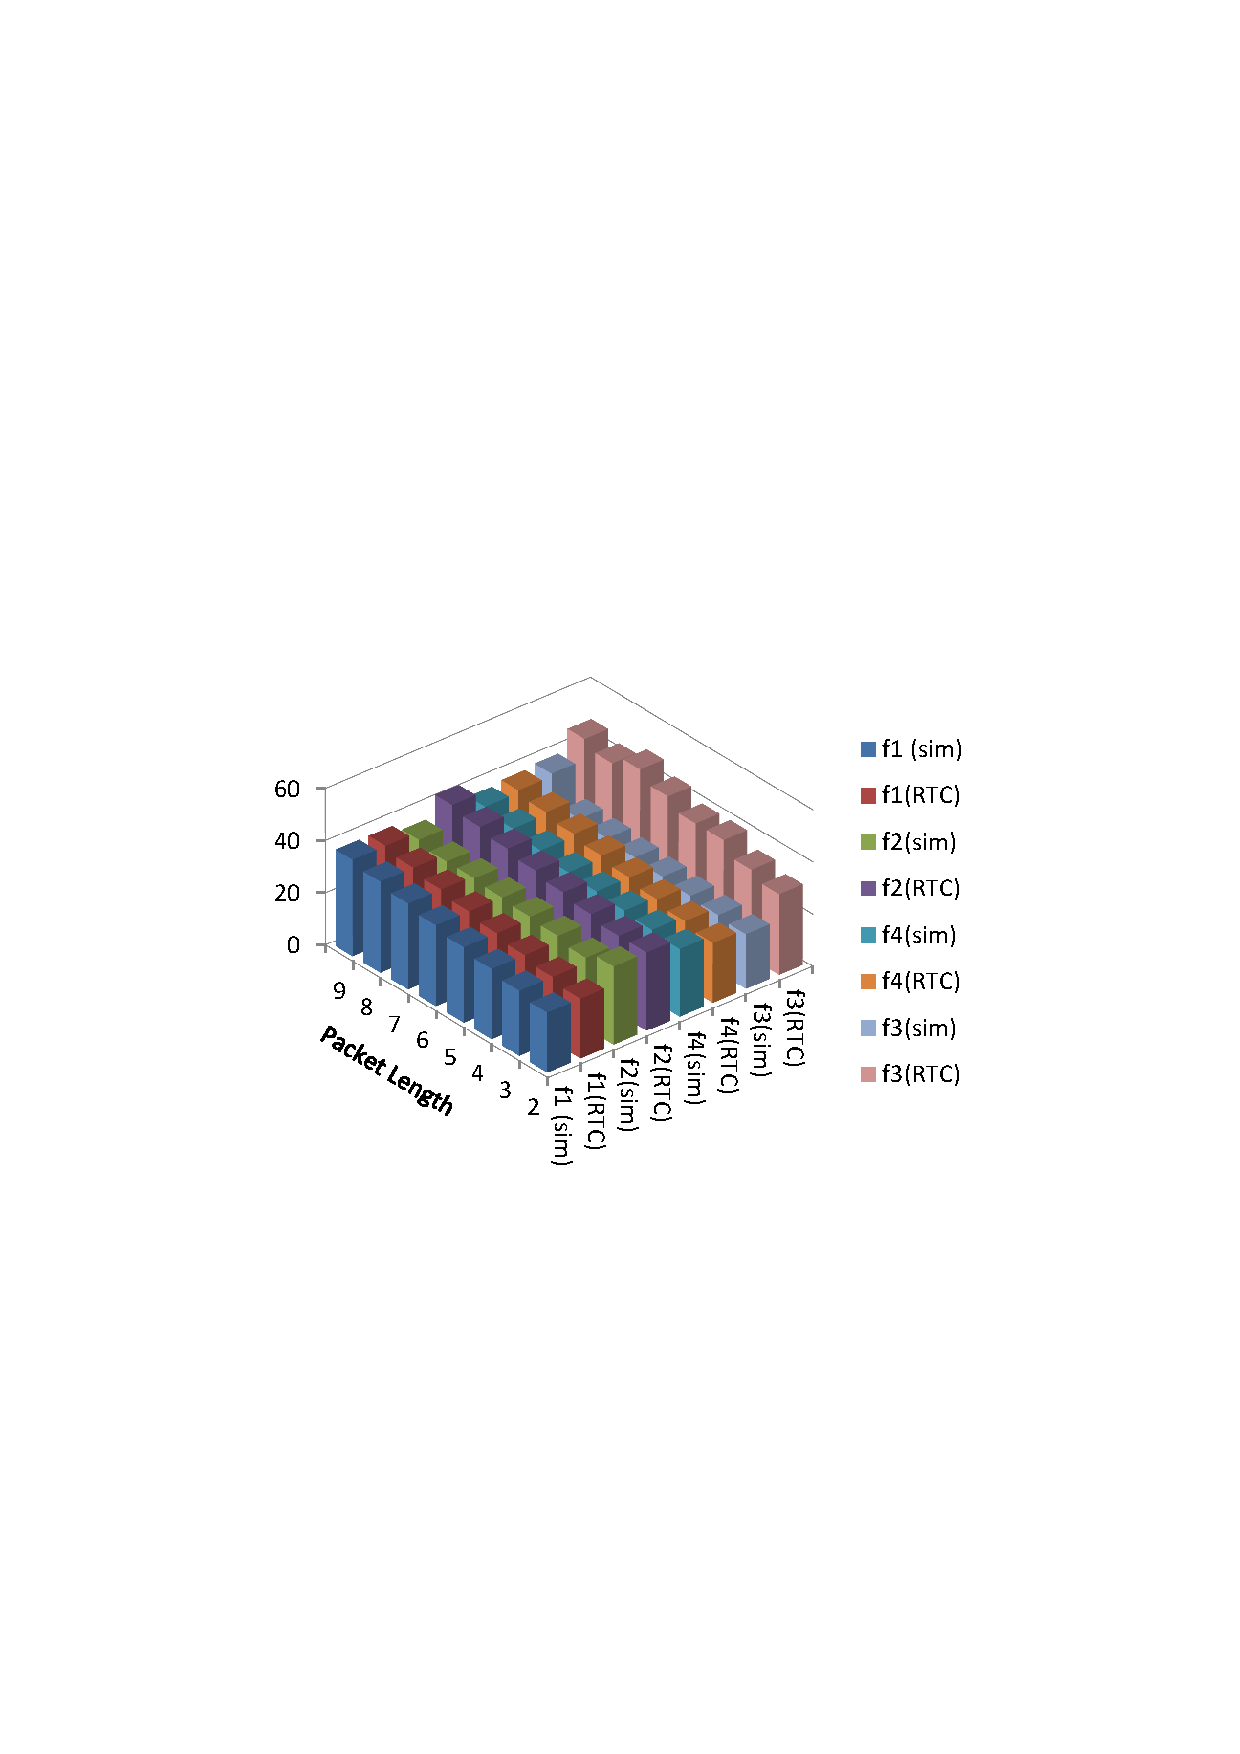
\includegraphics[scale=0.65]{figures/rtcvssim.pdf}\\
  \caption{Comparison with simulation}\label{rtcvssim}
\end{figure}

\section{Conclusion}\label{conclusion}
The priority-aware wormhole-switched NoC is a promising platform for the on-chip real-time communication if the worst-case performance can be accurately analyzed and guaranteed. Simulation is not well suited for this purpose because it is difficult to cover all the corner cases. In this paper, we propose an RTC based performance model to achieve this goal. We first build the traffic model and service model for this NoC, and propose a novel method to derive the upper service curve of credit-based flow control. Compared with the FLA and LLA methods which assume the router to be single cycle and free of flow control, our performance model is more general and comprehensive. Based on the proposed RTC model, we then proposed an end-to-end delay analysis algorithm and a buffer sizing algorithm. The delay analysis algorithm can be implemented to compute the end-to-end delay for each flow automatically, and verify whether all these flows meet their deadline under this configuration. To improve the calculated delay bound, we also proposed the concept of collapsible sub-path. The proposed buffer sizing algorithm can optimize the buffer size from high-priority flows to low-priority flows. It can also be implemented to perform the buffer reduction automatically under the constraint of deadline. Compared with the DNC based performance model, our model can give tighter performance bound, because the RTC-based model takes the upper service curve and lower arrival curve into consideration. Experimental results also illustrate that our method indeed outperforms the conventional analytical methods, e.g. LLA and DNC, when the tightness of performance bound are considered. Our results can be applied to the mapping, routing and power reduction of NoC.

\section*{Acknowledgement}
The authors would thank the reviewers for their suggestions and comments, and all the experiments are carried out at the Integrated Microsystem Lab (IML) of McGill University. This research is supported by High Technology Research and Development Program of China (Grant No. 2012AA012201, 2012AA011902).

\bibliographystyle{unsrt}
\bibliography{Docear}

\end{document}
